%Resultados

\section{Resultados}\label{sec:resultados}
\subsection{Parte 1. Amplificador de potencia} \label{subsec:parte1}

\begin{enumerate}
  \item \textbf{Mida los puntos de operación de todos los elementos activos, con el fin de verificar el correcto funcionamiento del circuito.}

        \begin{table}[H]
          \centering
          \begin{tabular}{|c|c|c|c|c|c|c|}
            \hline
            \textbf{Transistor} & \textbf{Vc[V]} & \textbf{$\Delta Vc[V]$} & \textbf{Vb[V]} & \textbf{$\Delta Vb[V]$} & \textbf{Ve[V]} & \textbf{$\Delta Ve[V]$} \\
            \hline
            Q4                  & 300m           & $\pm$ 20m               & 0m             & $\pm$ 20m               & -600m          & $\pm$ 40m               \\
            Q5                  & 10             & $\pm$ 1                 & 600m           & $\pm$ 40m               & 20m            & $\pm$ 4m                \\
            Q6                  & -10            & $\pm$ 1                 & -600m          & $\pm$ 40m               & 20m            & $\pm$ 4m                \\
            \hline
          \end{tabular}
          \caption{mediciones para hallar puntos de operación}
          \label{tab:pto_oper1}
        \end{table}

        Haciendo uso de las ecuaciones \ref{eqn:incertidumbre_vce} y \ref{eqn:incertidumbre_ic}, hallamos sus puntos de operación.

        \begin{itemize}
          \item $\mathbf{V_{CEQ}}$

                \begin{align*}
                  \Delta V_{CEQ_4} & = \sqrt{\left(\Delta V_C\right)^2 + \left(\Delta V_E\right)^2}     \\[0.2cm]
                  \Delta V_{CEQ_4} & = \sqrt{\left(0.04\right)^2 + \left(0.04\right)^2}=\pm 44.72m\volt \\[0.2cm]
                  \Delta V_{CEQ_5} & = \sqrt{\left(1\right)^2 + \left(0.02\right)^2}=\pm 1\volt         \\[0.2cm]
                  \Delta V_{CEQ_6} & = \sqrt{\left(1\right)^2 + \left(0.02\right)^2}=\pm 1\volt         \\[1cm]
                  V_{CEQ_4}        & =0.3-(-0.6)=0.9 \pm 0.04472\volt                                   \\[0.2cm]
                  V_{CEQ_5}        & =10-(0.02)=9.98 \pm 1\volt                                         \\[0.2cm]
                  V_{CEQ_6}        & =-10-(0.02)=-10.02 \pm 1\volt                                      \\[1cm]
                \end{align*}


          \item $\mathbf{I_{CQ}}$

                \begin{align*}
                  \Delta I_{c}   & = \sqrt{\left(\frac{\Delta V_{A}}{R}\right)^2 + \left(\frac{\Delta V_{B}}{R}\right)^2 + \left(\frac{(V_{A} - V_{B}) \cdot \Delta R}{R^2}\right)^2} \\[0.2cm]
                  \Delta I_{c5}  & = \sqrt{\left(\frac{1}{22k}\right)^2 + \left(\frac{0.04}{22k}\right)^2 + \left(\frac{(10-0.6) \cdot 0.05(22k)}{22k^2}\right)^2}                    \\[0.2cm]
                  \Delta I_{c_5} & =\Delta I_{c_6} =\pm 50.257\mu A                                                                                                                   \\[0.2cm]
                  \Delta I_{c_4} & = \sqrt{\left(\frac{1}{27k}\right)^2 + \left(\frac{0.02}{27k}\right)^2 + \left(\frac{(10-(0)) \cdot 0.05(27k)}{27k^2}\right)^2}                    \\[0.2cm]
                  \Delta I_{c_4} & =\pm 47.42\mu A                                                                                                                                    \\[1cm]
                  I_{CQ_4}       & =\dfrac{10-(0)}{27k}=370 \pm 47.42\mu A                                                                                                            \\[0.2cm]
                  I_{CQ_5}       & = I_{CQ_6}=\dfrac{10-(0.6)}{22k}=427.27 \pm 50.257\mu A                                                                                            \\[0.2cm]
                \end{align*}
        \end{itemize}

        \begin{table}[H]
          \centering
          \begin{tabular}{|c|c|c|c|c|c|c|}
            \hline
            \textbf{Transistores} & $v_{CE} [V]$ & $\Delta V_{CE} [V]$  & $E_{r_{V_{CE}}} [\%]$ & $I_{C} [\mu A]$ & $\Delta I_{C} [\mu A]$ & $E_{r_{I_{C}}} [\%]$ \\
            \hline
            $Q_4$                 & $0.9$        & $\pm 44.72 \text{m}$ & $30.77 \text{m}$      & $370$           & $\pm 47.42$            & $25.42$              \\
            \hline
            $Q_5$                 & $9.98$       & $\pm 1$              & $0.2$                 & $427.27$        & $\pm 50.257$           & $7.39$               \\
            \hline
            $Q_6$                 & $-10.02$     & $\pm 1$              & $0.2$                 & $427.27$        & $\pm 50.257$           & $7.39$               \\
            \hline
          \end{tabular}
          \caption{Mediciones indirectas con sus errores relativos de sus puntos de operación }
          \label{tab:puntos_operacion_experimental_maserror}
        \end{table}


  \item \textbf{Con ayuda del generador de funciones, determine el modelo circuital a pequeña señal y a frecuencias medias (1kHz aprox.) de la EP.}

        \begin{table}[H]
          \centering
          \begin{tabular}{|c|c|c|c|c|c|c|}
            \hline
            \textbf{Vi[V\_p]} & $\mathbf{\Delta Vi[V\_p]}$ & \textbf{Vo[V\_p]} & $\mathbf{\Delta Vo[V\_p]}$ & \textbf{A[V/V]} & $\mathbf{\Delta A[V/V]}$ \\
            \hline
            1                 & $\pm$ 0.1                  & 1                 & $\pm$ 0.1                  & 1               & $\pm$ 141.42 m           \\
            \hline
          \end{tabular}
          \caption{Mediciones de ganancia en la etapa de potencia (EP)}
          \label{tab:ganancia_ep}
        \end{table}

        En la tabla \ref{tab:ganancia_ep} se hallo el $\mathbf{\Delta A[V/V]}$ gracias a la ecuación \ref{eqn:incertidumbre_av}

        \begin{table}[H]
          \centering
          \begin{tabular}{|c|c|}
            \hline
            $E_{r_{A_v}} [\%]$ & 2.77 \\
            \hline
          \end{tabular}
          \caption{Error porcentual de la ganancia}
          \label{tab:error_porcentual1_av}
        \end{table}


        \begin{itemize}
          \item \textbf{Impedancia de entrada}
                Acá sacamos las incertidumbres gracias a la ecuación \ref{eqn:incertidumbre}.

                \begin{table}[H]
                  \centering
                  \begin{tabular}{|c|c|c|c|c|c|c|c|}
                    \hline
                    $\mathbf{V_g[V_p]}$ & $\mathbf{\Delta V_g[V_p]}$ & $\mathbf{V_i[V_p]}$ & $\mathbf{\Delta V_i[V_p]}$ & $\mathbf{R_p[\Omega]}$ & $\mathbf{\Delta R_p[\%]}$ & $\mathbf{Z_{in}[\Omega]}$ & $\mathbf{\Delta Z_{in}[\Omega]}$ \\
                    \hline
                    1                   & 0.1                        & 0.5                 & 0.1                        & $11 k +50$             & $1\%$                     & $11k$                     & $\pm 4.92k$                      \\
                    \hline
                  \end{tabular}
                  \caption{Medición de impedancias de entrada}
                  \label{tab:med_zin_ep}
                \end{table}

                \begin{table}[H]
                  \centering
                  \begin{tabular}{|c|c|}
                    \hline
                    $E_{r_{Z_{in}}} [\%]$ & 3.19 \\
                    \hline
                  \end{tabular}
                  \caption{Error porcentual de la impedancia de entrada}
                  \label{tab:error_porcentual1_zin}
                \end{table}

          \item \textbf{Impedancias de salida}

                \begin{table}[H]
                  \centering
                  \begin{tabular}{|c|c|c|c|c|c|c|c|}
                    \hline
                    \textbf{Vo\_sc[V\_p]} & $\mathbf{\Delta vo\_sc[V\_p]}$ & \textbf{Vo\_cc[V\_p]} & $\mathbf{\Delta Vo\_cc[V\_p]}$ & \textbf{Rp[$\Omega$]} & $\mathbf{\Delta Rp[\Omega]}$ & \textbf{Zo[$\Omega$]} & $\mathbf{\Delta Zo[\Omega]}$ \\
                    \hline
                    1                     & 0.1                            & 0.9                   & 0.1                            & 180                   & 5\%                          & 20                    & $\pm$ 29.91                  \\
                    \hline
                  \end{tabular}
                  \caption{Medición de impedancia de salida}
                  \label{tab:med_zo_ep}
                \end{table}
        \end{itemize}

        \begin{table}[H]
          \centering
          \begin{tabular}{|c|c|}
            \hline
            $E_{r_{Z_{o}}} [\%]$ & 73.18 \\
            \hline
          \end{tabular}
          \caption{Error porcentual de la impedancia de salida}
          \label{tab:error_porcentual1_zo}
        \end{table}


  \item \textbf{Modificando la polarización de la etapa, conviértala en:}
        \begin{enumerate}
          \item \textbf{Un amplificador clase B, colocando los transistores
                  de potencia justo en la zona de corte.}

                En la siguiente imagen se muestra el efecto de cruce, debido a la manipulación de la resistencia variable o potenciómetro.

                \begin{figure}[H]
                  \centering
                  \renewcommand{\figurename}{Imagen}
                  \setcounter{figure}{0}
                  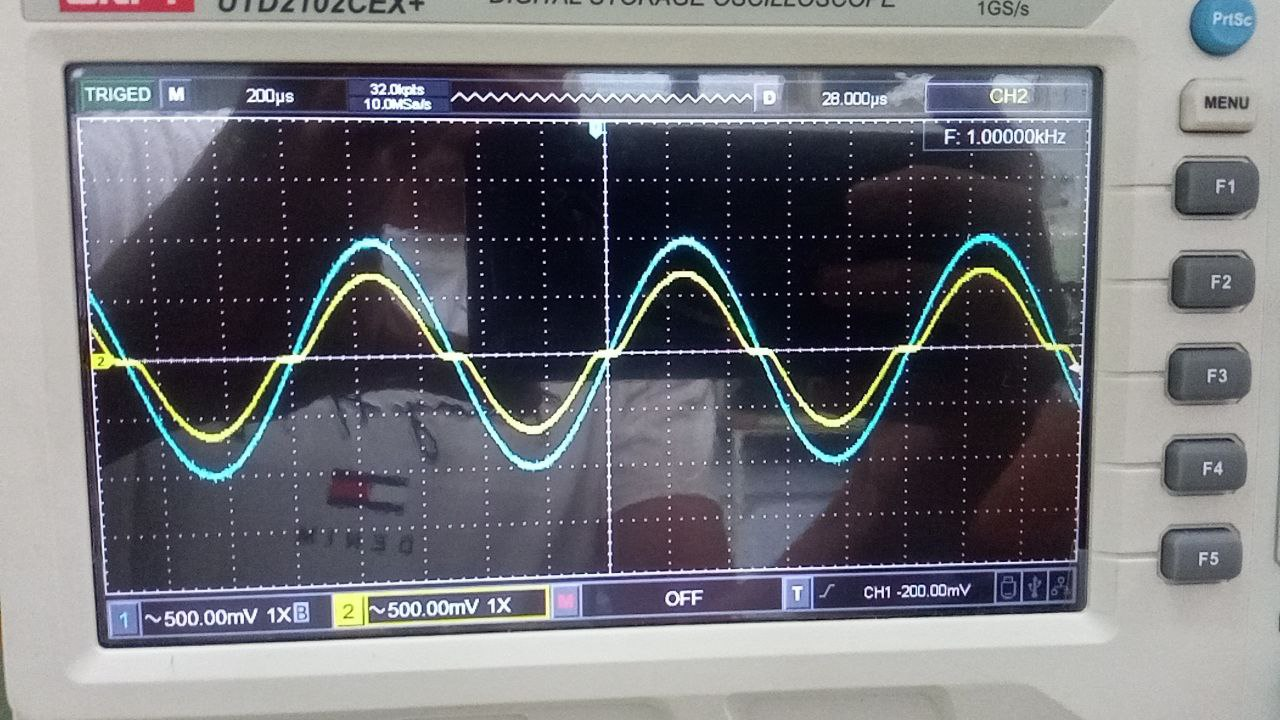
\includegraphics[width=\textwidth]{Imagenes/crossover_b.jpg}
                  \caption{Efecto crossover en un amplificador Tipo B. Siendo X=0.56}
                  \label{fig:crossover_b}
                \end{figure}

                \begin{table}[H]
                  \centering
                  \begin{tabular}{|c|c|c|c|}
                    \hline
                    \textbf{time/div} $[\mu s]$ & \textbf{Channel} & \textbf{voltios/div $[\volt]$} & \textbf{Acoplamiento} \\ \hline
                    $200 \, \pm 40 \,  $        & 1 (Azul)         & $500 \pm 100 \text{m}  $       & AC                    \\ \hline
                    $200 \, \pm 40 \,  $        & 2 (Amarillo)     & $500 \pm 100 \text{m}   $      & AC                    \\ \hline
                  \end{tabular}
                  \caption{Escalas Usada en el Osciloscopio Digital UNI-T UTD2102CEX+}
                  \label{tab:escala_crossover_b}
                \end{table}


          \item \textbf{Un amplificador clase AB, colocando los transistores de potencia conduciendo con corriente pequeñas.}

                \begin{figure}[H]
                  \centering
                  \renewcommand{\figurename}{Imagen}
                  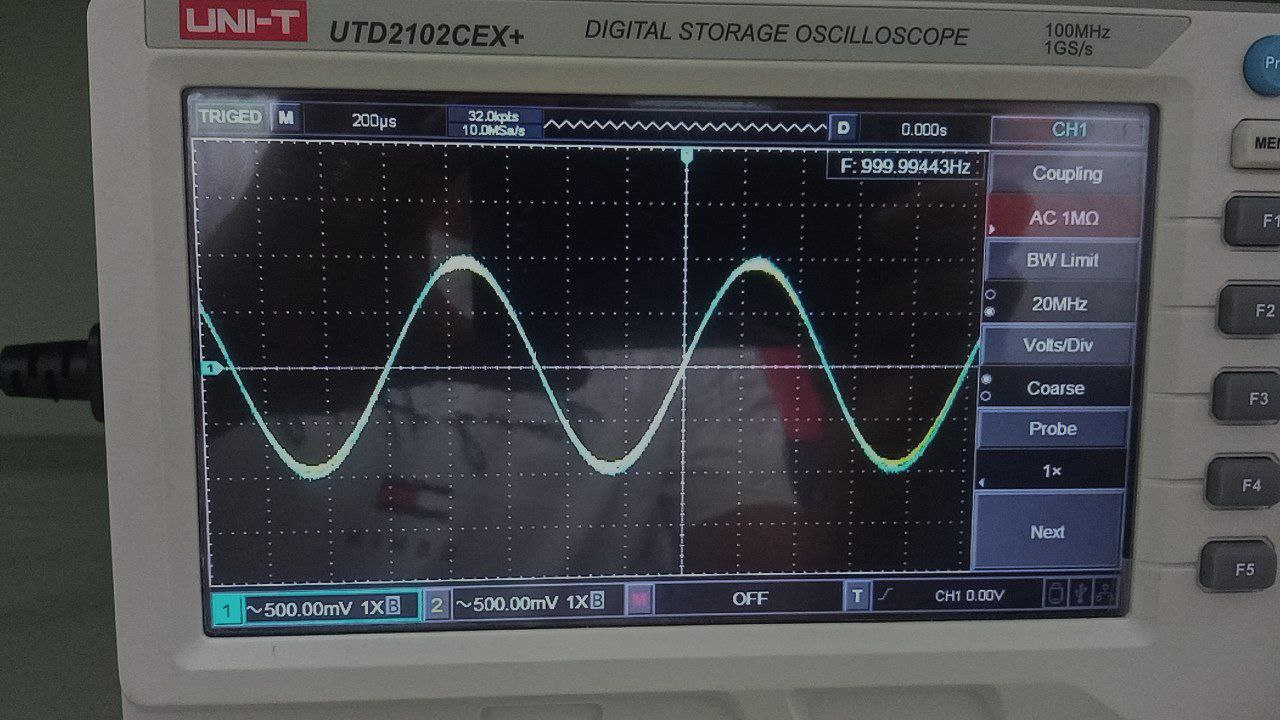
\includegraphics[width=\textwidth]{Imagenes/sincrossover.jpg}
                  \caption{Sin Efecto crossover Se convierte en un amplificador Tipo AB. Siendo X=0.5}
                  \label{fig:sincrossover}
                \end{figure}


                \begin{table}[H]
                  \centering
                  \begin{tabular}{|c|c|c|c|}
                    \hline
                    \textbf{time/div} $[\mu s]$ & \textbf{Channel} & \textbf{voltios/div $[\volt]$} & \textbf{Acoplamiento} \\ \hline
                    $200 \, \pm 40 \, $         & 1 (Azul)         & $500 \pm 100 \text{m}  $       & AC                    \\ \hline
                    $200 \, \pm 40 \,   $       & 2 (Amarillo)     & $500  \pm 100 \text{m}   $     & AC                    \\ \hline
                  \end{tabular}
                  \caption{Escalas Usada en el Osciloscopio Digital UNI-T UTD2102CEX+}
                  \label{tab:escala_sincrossover}
                \end{table}
        \end{enumerate}
\end{enumerate}

\subsection{Parte 2. Amplificador Diferencial} \label{subsec:parte2}

\begin{enumerate}
  \item \textbf{Mida los puntos de operación de todos los elementos activos, con el fin de verificar el correcto funcionamiento del circuito.}

        \begin{table}[H]
          \centering
          \begin{tabular}{|c|c|c|c|c|c|c|}
            \hline
            \textbf{Transistor} & $\mathbf{Vc[V]}$ & $\mathbf{\Delta Vc[V]}$ & $\mathbf{Vb[V]}$ & $\mathbf{\Delta Vb[V]}$ & $\mathbf{Ve[V]}$ & $\mathbf{\Delta Ve[V]}$ \\
            \hline
            Q1                  & 8                & $\pm$ 1                 & -120m            & $\pm$ 20m               & -700m            & $\pm$ 100m              \\
            \hline
            Q2                  & 7.2              & $\pm$ 0.4               & -60m             & $\pm$ 10m               & -680m            & $\pm$ 40m               \\
            \hline
          \end{tabular}
          \caption{Mediciones para hallar punto de operación}
          \label{tab:pto_ope_ed}
        \end{table}
        Haciendo uso de las ecuaciones \ref{eqn:incertidumbre_vce} y \ref{eqn:incertidumbre_ic}, hallamos sus puntos de operación e incertidumbres.

        \begin{itemize}
          \item $\mathbf{V_{CEQ}}$

                \begin{align*}
                  \Delta V_{CEQ_1} & = \sqrt{\left(\Delta V_C\right)^2 + \left(\Delta V_E\right)^2}   \\[0.2cm]
                  \Delta V_{CEQ_1} & = \sqrt{\left(1\right)^2 + \left(0.1\right)^2}=\pm 1.005 \volt   \\[0.2cm]
                  \Delta V_{CEQ_2} & = \sqrt{\left(0.4\right)^2 + \left(0.04\right)^2}=\pm 0.402\volt \\[1cm]
                  V_{CEQ_1}        & =8-(-0.7)=8.7 \pm 1.005\volt                                     \\[0.2cm]
                  V_{CEQ_2}        & =7.2-(-0.68)=7.88 \pm 0.402\volt                                 \\[1cm]
                \end{align*}


          \item $\mathbf{I_{CQ}}$

                \begin{align*}
                  \Delta I_{c}   & = \sqrt{\left(\frac{\Delta V_{A}}{R}\right)^2 + \left(\frac{\Delta V_{B}}{R}\right)^2 + \left(\frac{(V_{A} - V_{B}) \cdot \Delta R}{R^2}\right)^2} \\[0.2cm]
                  \Delta I_{c1}  & = \sqrt{\left(\frac{1}{4.7k}\right)^2 + \left(\frac{1}{4.7k}\right)^2 + \left(\frac{(10-8) \cdot 0.05(4.7k)}{4.7k^2}\right)^2}                     \\[0.2cm]
                  \Delta I_{c_1} & =\pm 301.648\mu A                                                                                                                                  \\[1cm]
                  \Delta I_{c2}  & = \sqrt{\left(\frac{1}{4.7k}\right)^2 + \left(\frac{0.4}{4.7k}\right)^2 + \left(\frac{(10-7.2) \cdot 0.05(4.7k)}{4.7k^2}\right)^2}                 \\[0.2cm]
                  \Delta I_{c_2} & =\pm 231.084 \mu A                                                                                                                                 \\[1cm]
                  I_{CQ_1}       & =\dfrac{10-(8)}{4.7k}=425.532 \pm 301.648\mu A                                                                                                     \\[1cm]
                  I_{CQ_2}       & =\dfrac{10-(7.2)}{4.7k}=595.745 \pm 231.084\mu A                                                                                                   \\[1cm]
                \end{align*}

        \end{itemize}

        \begin{table}[H]
          \centering
          \begin{tabular}{|c|c|c|c|c|c|c|}
            \hline
            \textbf{Transistores} & $v_{CE} [V]$ & $\Delta V_{CE} [V]$ & $E_{r_{V_{CE}}} [\%]$ & $I_{C} [\mu A]$ & $\Delta I_{C} [\mu A]$ & $E_{r_{I_{C}}} [\%]$ \\
            \hline
            $Q_1$                 & $8.7$        & $\pm 1.005 $        & $8.75$                & $425.532$       & $\pm 301.648$          & $29.76$              \\
            \hline
            $Q_2$                 & $7.88$       & $\pm 0.402$         & $1.5$                 & $595.745$       & $\pm 231.084$          & $1.66$               \\
            \hline
          \end{tabular}
          \caption{Mediciones indirectas con sus errores relativos de sus puntos de operación }
          \label{tab:puntos_operacion_experimental_maserror_parte2}
        \end{table}

  \item \textbf{Con la metodología expuesta por Ud. en el trabajo de preparación, determine el modelo completo del amplificador diferencial.}
        \begin{table}[H]
          \centering
          \begin{tabular}{|c|c|c|c|c|c|}
            \hline
            \textbf{Vi[V\textsubscript{p}]} & \textbf{\(\Delta\)Vi[V\textsubscript{p}]} & \textbf{Vo[V\textsubscript{p}]} & \textbf{\(\Delta\)Vo[V\textsubscript{p}]} & \textbf{$A_d$[V/V]} & \textbf{\(\Delta\)$A_d$[V/V]} \\\hline
            1                               & \(\pm\) 0.2                               & 3                               & \(\pm\) 0.2                               & 3                   & \(\pm\) 632.46m               \\\hline
          \end{tabular}
          \caption{Mediciones de ganancia en modo diferencial de la Etapa diferencial (ED)}
          \label{tab:ganancia_ed}
        \end{table}

        \begin{table}[H]
          \centering
          \begin{tabular}{|c|c|}
            \hline
            $E_{r_{A_d}} [\%]$ & 1.70 \\
            \hline
          \end{tabular}
          \caption{Error porcentual de la ganancia en modo diferencial}
          \label{tab:error_porcentual2_ad}
        \end{table}

        \begin{table}[H]
          \centering
          \begin{tabular}{|c|c|c|c|c|c|}
            \hline
            \textbf{Vi[V\textsubscript{p}]} & \textbf{\(\Delta\)Vi[V\textsubscript{p}]} & \textbf{Vo[V\textsubscript{p}]} & \textbf{\(\Delta\)Vo[V\textsubscript{p}]} & \textbf{$A_c$ [V/V]} & \textbf{\(\Delta\)$A_c$[V/V]} \\\hline
            1                               & \(\pm\) 0.2                               & 300m                            & \(\pm\) 20m                               & 0.3                  & \(\pm\) 208.81m               \\\hline
          \end{tabular}
          \caption{Mediciones de ganancia en modo común de la Etapa diferencial (ED)}
          \label{tab:ganancia_ed_modo_comun}
        \end{table}


        \begin{table}[H]
          \centering
          \begin{tabular}{|c|c|}
            \hline
            $E_{r_{A_c}} [\%]$ & 3.23 \\
            \hline
          \end{tabular}
          \caption{Error porcentual de la ganancia en modo común}
          \label{tab:error_porcentual2_ac}
        \end{table}

        \begin{table}[H]
          \centering
          \begin{tabular}{|c|c|c|}
            \hline
            CMRR $(\rho) [dB]$ & $\Delta$ CMRR $(\rho) [dB]$ & $E_{r_{\rho}} [\%]$ \\
            \hline
            20                 & $\pm 14.55$                 & $2.20$              \\
            \hline
          \end{tabular}
          \caption{Medida indirecta del CMRR de la ED}
          \label{tab:medida_indirecta_cmrr_ed}
        \end{table}


        \begin{table}[H]
          \centering
          \begin{tabular}{|c|c|c|c|c|c|c|c|}
            \hline
            \textbf{Vg[V\textsubscript{p}]} & \textbf{\(\Delta\)Vg[V\textsubscript{p}]} & \textbf{Vi[V\textsubscript{p}]} & \textbf{\(\Delta\)Vi[V\textsubscript{p}]} & \textbf{Rp[Ω]} & \textbf{\(\Delta\)Rp[Ω]} & \textbf{Zd[Ω]} & \textbf{\(\Delta\)Zd[Ω]} \\\hline
            1                               & \(\pm\) 0.2                               & 0.44                            & \(\pm\) 0.04                              & 39k            & \(\pm\) 5\%              & 30.64k         & \(\pm\) 12.119k          \\\hline
          \end{tabular}
          \caption{Medición de impedancia de entrada en modo diferencial}
          \label{tab:impedancia_entrada_diferencial}
        \end{table}


        \begin{table}[H]
          \centering
          \begin{tabular}{|c|c|}
            \hline
            $E_{r_{Z_{d}}} [\%]$ & 25.92 \\
            \hline
          \end{tabular}
          \caption{Error porcentual de la impedancia de entrada en modo diferencial}
          \label{tab:error_porcentual2_zd}
        \end{table}


        \begin{table}[H]
          \centering
          \begin{tabular}{|c|c|c|c|c|c|c|c|}
            \hline
            \textbf{Vg[V\textsubscript{p}]} & \textbf{\(\Delta\)Vg[V\textsubscript{p}]} & \textbf{Vi[V\textsubscript{p}]} & \textbf{\(\Delta\)Vi[V\textsubscript{p}]} & \textbf{Rp[Ω]} & \textbf{\(\Delta\)Rp[Ω]} & \textbf{Zc[Ω]} & \textbf{\(\Delta\)Zc[Ω]} \\\hline
            1                               & \(\pm\) 0.2                               & 0.32                            & \(\pm\) 0.02                              & 47k            & \(\pm\) 5\%              & 44.24k         & \(\pm\) 13.809k          \\\hline
          \end{tabular}
          \caption{Medición de impedancias de entrada en modo común}
          \label{tab:impedancias_entrada_comun}
        \end{table}

        \begin{table}[H]
          \centering
          \begin{tabular}{|c|c|}
            \hline
            $E_{r_{Z_{c}}} [\%]$ & 9.44 \\
            \hline
          \end{tabular}
          \caption{Error porcentual de la impedancia de entrada en modo común}
          \label{tab:error_porcentual2_zc}
        \end{table}


        \begin{table}[H]
          \centering
          \begin{tabular}{|c|c|c|c|c|c|c|c|}
            \hline
            \textbf{Vo\_sc[V\textsubscript{p}]} & \textbf{\(\Delta\)vo\_sc[V\textsubscript{p}]} & \textbf{Vo\_cc[V\textsubscript{p}]} & \textbf{\(\Delta\)Vo\_cc[V\textsubscript{p}]} & \textbf{Rp[Ω]} & \textbf{\(\Delta\)Rp[Ω]} & \textbf{Zo[Ω]} & \textbf{\(\Delta\)Zo[Ω]} \\\hline
            3                                   & \(\pm\) 0.2                                   & 1.4                                 & \(\pm\) 0.1                                   & 4.7k           & \(\pm\) 5\%              & 5.37k          & \(\pm\) 1.02k            \\\hline
          \end{tabular}
          \caption{Medición de impedancia de salida}
          \label{tab:impedancias_salida}
        \end{table}


        \begin{table}[H]
          \centering
          \begin{tabular}{|c|c|}
            \hline
            $E_{r_{Z_{o}}} [\%]$ & 14.26 \\
            \hline
          \end{tabular}
          \caption{Error porcentual de la impedancia de salida}
          \label{tab:error_porcentual2_zo}
        \end{table}


  \item \textbf{Determine los limites de excursión: en modo diferencial
          y en modo común. en cada caso dibuje o fotografié las señales de salida (ambas salidas asimétricas) en máxima excursión.}

        \begin{figure}[H]
          \centering
          \renewcommand{\figurename}{Imagen}
          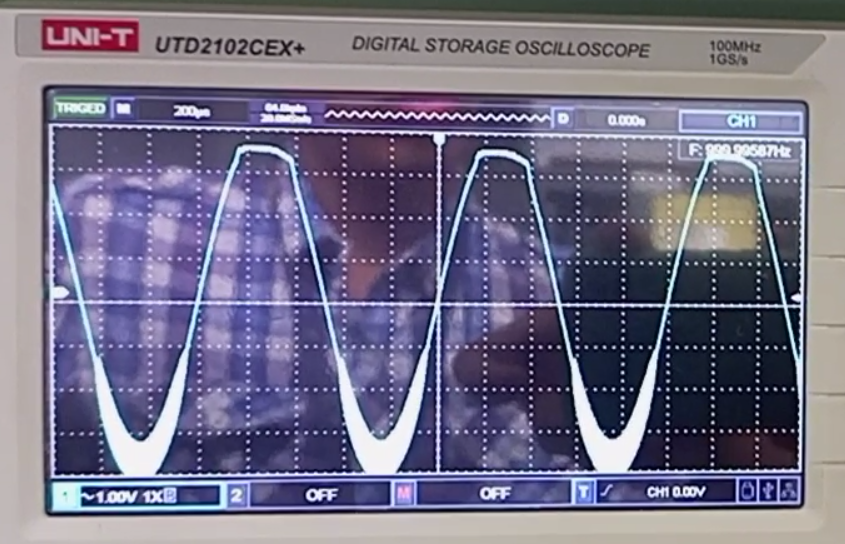
\includegraphics[width=\textwidth]{Imagenes/vod.png}
          \caption{Limite de excursión en modo diferencial.}
          \label{fig:vod}
        \end{figure}

        \begin{table}[H]
          \centering
          \begin{tabular}{|c|c|c|c|}
            \hline
            \textbf{time/div} $[\mu s]$ & \textbf{Channel} & \textbf{voltios/div $[\volt]$} & \textbf{Acoplamiento} \\ \hline
            $200 \, \pm 40 \, $         & 1 (Azul)         & $1 \pm 0.2  $                  & AC                    \\ \hline
          \end{tabular}
          \caption{Escalas Usada en el Osciloscopio Digital UNI-T UTD2102CEX+}
          \label{tab:escala_lim_mododif}
        \end{table}

        \begin{table}[H]
          \centering
          \begin{tabular}{|c|c|}
            \hline
            $\mathbf{V_i > 2.2 V_p}$ & $\mathbf{-3.9V_p <V_o<3.9V_p}$ \\
            \hline
          \end{tabular}
          \caption{Limites de excursión de la etapa diferencial en modo diferencial}
          \label{tab:exp_lim_exc_modif}
        \end{table}



        \begin{figure}[H]
          \centering
          \renewcommand{\figurename}{Imagen}
          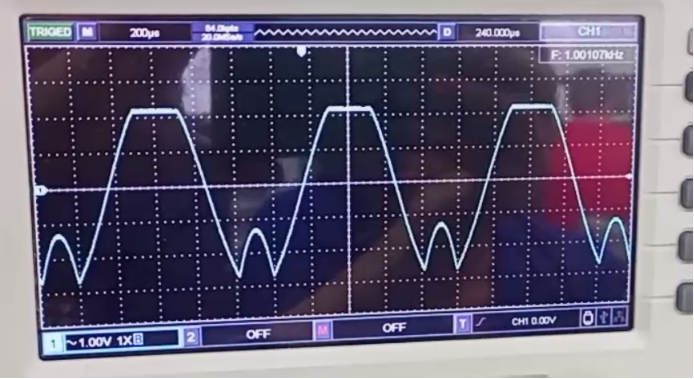
\includegraphics[width=\textwidth]{Imagenes/voc.png}
          \caption{Limite de excursión en modo común.}
          \label{fig:voc}
        \end{figure}


        \begin{table}[H]
          \centering
          \begin{tabular}{|c|c|c|c|}
            \hline
            \textbf{time/div} $[\mu s]$ & \textbf{Channel} & \textbf{voltios/div $[\volt]$} & \textbf{Acoplamiento} \\ \hline
            $200 \, \pm 40 \, $         & 1 (Azul)         & $1 \pm 0.2  $                  & AC                    \\ \hline
          \end{tabular}
          \caption{Escalas Usada en el Osciloscopio Digital UNI-T UTD2102CEX+}
          \label{tab:escala_lim_modocomun}
        \end{table}

        \begin{table}[H]
          \centering
          \begin{tabular}{|c|c|}
            \hline
            $\mathbf{V_i > 12 V_p}$ & $\mathbf{-2.4V_p <V_o<2.4V_p}$ \\
            \hline
          \end{tabular}
          \caption{Límites de excursión de la etapa diferencial en modo común}
          \label{tab:exp_lim_exc_mocom}
        \end{table}

\end{enumerate}

\subsection{Parte 3. Amplificador multietapas} \label{subsec:parte3}

\begin{enumerate}

  \item \textbf{Determine experimentalmente para cada etapa desacoplada,
          los puntos de operación de los elementos activos y los modelos dinámicos de cada etapa.}

        \begin{table}[H]
          \centering
          \begin{tabular}{|c|c|c|c|c|c|c|}
            \hline
            \textbf{Transistor} & \textbf{Vc[V]} & $\mathbf{\Delta Vc[V]}$ & \textbf{Vb[V]} & $\mathbf{\Delta Vb[V]}$ & \textbf{Ve[V]} & $\mathbf{\Delta Ve[V]}$ \\ \hline
            Q1                  & 7.2            & $\pm 0.4$               & 240m           & $\pm 20m$               & -360m          & $\pm 100m$              \\ \hline
            Q2                  & 7.2            & $\pm 0.4$               & 260m           & $\pm 20m$               & -360m          & $\pm 20m$               \\ \hline
            Q3                  & 5.2            & $\pm 0.4$               & 8              & $\pm 0.4$               & 9              & $\pm 1$                 \\ \hline
            Q4                  & 900m           & $\pm 100m$              & 360m           & $\pm 20m$               & -200m          & $\pm 20m$               \\ \hline
            Q5                  & 10             & $\pm 1$                 & 900m           & $\pm 100m$              & 380m           & $\pm 20m$               \\ \hline
            Q6                  & -10            & $\pm 1$                 & -220m          & $\pm 20m$               & 360m           & $\pm 20m$               \\ \hline
          \end{tabular}
          \caption{Mediciones para hallar punto de operación, acoplando sus etapas}
          \label{tab:punto_operacion_aco}
        \end{table}



        Haciendo uso de las ecuaciones \ref{eqn:incertidumbre_vce} y \ref{eqn:incertidumbre_ic}, hallamos sus puntos de operación e incertidumbres (Acoplado).

        \begin{itemize}
          \item $\mathbf{V_{CEQ}}$

                \begin{align*}
                  V_{CEQ_3} & =5.2-(9)=-3.8 \pm 1.08\volt    \\[0.2cm]
                  V_{CEQ_1} & =7.2-(0.36)=7.56 \pm 0.41\volt \\[0.2cm]
                  V_{CEQ_2} & =7.2-(0.36)=7.56 \pm 0.41\volt \\[0.2cm]
                  V_{CEQ_4} & =0.9-(-0.2)=1.1 \pm 0.10\volt  \\[0.2cm]
                  V_{CEQ_5} & =10-(0.38)=9.62 \pm 1\volt     \\[0.2cm]
                  V_{CEQ_6} & =-10-(0.36)=-10.36 \pm 1\volt  \\[1cm]
                \end{align*}


          \item $\mathbf{I_{CQ}}$

                \begin{align*}
                  I_{CQ_3} & =\dfrac{9-(-10)}{6.8k}=2.79 \pm 0.25 mA                   \\[0.2cm]
                  I_{CQ_4} & =\dfrac{10-(-0.36)}{5k}=357.04 \pm 47.12\mu A             \\[0.2cm]
                  I_{CQ_5} & =\dfrac{10-(0.9)}{22k}=413.64 \pm 50.14\mu A              \\[0.2cm]
                  I_{CQ_6} & =\dfrac{-0.22-(-10)}{22k}=444.55 \pm 50.61\mu A           \\[0.2cm]
                  I_{CQ_1} & = I_{CQ_2}=\dfrac{10-(7.2)}{4.7k}=595.74 \pm 231.08 \mu A \\[1cm]
                \end{align*}



                \begin{table}[H]
                  \centering
                  \begin{tabular}{|c|c|c|c|c|c|c|}
                    \hline
                    \textbf{Transistores} & $v_{CE} [V]$ & $\Delta V_{CE} [V]$ & $E_{r_{V_{CE}}} [\%]$ & $I_{C} [\mu A]$ & $\Delta I_{C} [\mu A]$ & $E_{r_{I_{C}}} [\%]$ \\
                    \hline
                    $Q_1$                 & $7.56$       & $\pm 0.41 $         & $5.5$                 & $595.74$        & $\pm 231.08$           & $1.67$               \\
                    \hline
                    $Q_2$                 & $7.56$       & $\pm 0.40 $         & $5.5$                 & $595.74$        & $\pm 231.08$           & $1.67$               \\
                    \hline
                    $Q_3$                 & $-3.8$       & $\pm 1.08$          & $17.48$               & $2790$          & $\pm 250$              & $24.55$              \\
                    \hline
                    $Q_4$                 & $1.1$        & $\pm 0.10$          & $15.38$               & $357.04$        & $\pm 47.12$            & $21.03$              \\
                    \hline
                    $Q_5$                 & $9.62$       & $\pm 1.00$          & $3.8$                 & $413.64$        & $\pm 50.14$            & $3.96$               \\
                    \hline
                    $Q_6$                 & $-10.36$     & $\pm 1.00$          & $3.6$                 & $444.55$        & $\pm 50.61$            & $11.73$              \\
                    \hline
                  \end{tabular}
                  \caption{Mediciones indirectas con sus errores relativos de sus puntos de operación Acoplados}
                  \label{tab:puntos_operacion_experimental_maserror_parte3}
                \end{table}

                \begin{table}[H]
                  \centering
                  \begin{tabular}{|c|c|c|c|c|c|c|}
                    \hline
                    \textbf{Transistor} & \textbf{Vc[V]} & $\mathbf{\Delta Vc[V]}$ & \textbf{Vb[V]} & $\mathbf{\Delta Vb[V]}$ & \textbf{Ve[V]} & $\mathbf{\Delta Ve[V]}$ \\ \hline
                    Q1                  & 7.2            & $\pm 0.4$               & 240m           & $\pm 20m$               & -400m          & $\pm 100m$              \\ \hline
                    Q2                  & 7.2            & $\pm 0.4$               & 240m           & $\pm 20m$               & -360m          & $\pm 20m$               \\ \hline
                    Q3                  & 5.2            & $\pm 0.4$               & 8              & $\pm 0.4$               & 9              & $\pm 1$                 \\ \hline
                    Q4                  & 900m           & $\pm 100m$              & 360m           & $\pm 20m$               & -300m          & $\pm 100m$              \\ \hline
                    Q5                  & 10             & $\pm 1$                 & 900m           & $\pm 100m$              & 360m           & $\pm 20m$               \\ \hline
                    Q6                  & -10            & $\pm 1$                 & -240m          & $\pm 20m$               & 360m           & $\pm 20m$               \\ \hline
                  \end{tabular}
                  \caption{Mediciones para hallar punto de operación, desacoplando sus etapas, colocando un jumper en C2, C5, y C7}
                  \label{tab:punto_operacion_desaco}
                \end{table}




                Haciendo uso de las ecuaciones \ref{eqn:incertidumbre_vce} y \ref{eqn:incertidumbre_ic}, hallamos sus puntos de operación e incertidumbres (Desacoplado).

                En este caso, solo varia en desacople $V_{b_6}$, $V_{e_1}$, $V_{e_4}$ y $V_{e_5}$, sabiendo eso, solo se modificaran dichos valores que sean afectados por estos parámetros.
          \item $\mathbf{V_{CEQ}}$

                \begin{align*}
                  V_{CEQ_3} & =5.2-(9)=-3.8 \pm 1.08\volt    \\[0.2cm]
                  V_{CEQ_1} & =7.2-(-0.4)=7.6 \pm 0.41\volt  \\[0.2cm]
                  V_{CEQ_2} & =7.2-(0.36)=7.56 \pm 0.41\volt \\[0.2cm]
                  V_{CEQ_4} & =0.9-(-0.3)=1.2 \pm 0.14\volt  \\[0.2cm]
                  V_{CEQ_5} & =10-(0.36)=9.64 \pm 1\volt     \\[0.2cm]
                  V_{CEQ_6} & =-10-(0.36)=-10.36 \pm 1\volt  \\[1cm]
                \end{align*}


          \item $\mathbf{I_{CQ}}$

                \begin{align*}
                  I_{CQ_3} & =\dfrac{9-(-10)}{6.8k}=2.79 \pm 0.25 mA                   \\[0.2cm]
                  I_{CQ_4} & =\dfrac{10-(-0.36)}{5k}=357.04 \pm 47.12\mu A             \\[0.2cm]
                  I_{CQ_5} & =\dfrac{10-(0.9)}{22k}=413.64 \pm 50.14\mu A              \\[0.2cm]
                  I_{CQ_6} & =\dfrac{-0.24-(-10)}{22k}=443.64 \pm 50.61\mu A           \\[0.2cm]
                  I_{CQ_1} & = I_{CQ_2}=\dfrac{10-(7.2)}{4.7k}=595.74 \pm 231.08 \mu A \\[1cm]
                \end{align*}



                \begin{table}[H]
                  \centering
                  \begin{tabular}{|c|c|c|c|c|c|c|}
                    \hline
                    \textbf{Transistores} & $v_{CE} [V]$ & $\Delta V_{CE} [V]$ & $E_{r_{V_{CE}}} [\%]$ & $I_{C} [\mu A]$ & $\Delta I_{C} [\mu A]$ & $E_{r_{I_{C}}} [\%]$ \\
                    \hline
                    $Q_1$                 & $7.6$        & $\pm 0.41 $         & $5$                   & $595.74$        & $\pm 231.08$           & $1.67$               \\
                    \hline
                    $Q_2$                 & $7.56$       & $\pm 0.40 $         & $5.5$                 & $595.74$        & $\pm 231.08$           & $1.67$               \\
                    \hline
                    $Q_3$                 & $-3.8$       & $\pm 1.08$          & $17.48$               & $2790$          & $\pm 250$              & $24.55$              \\
                    \hline
                    $Q_4$                 & $1.2$        & $\pm 0.14$          & $7.69$                & $357.04$        & $\pm 47.12$            & $21.03$              \\
                    \hline
                    $Q_5$                 & $9.64$       & $\pm 1.00$          & $3.6$                 & $413.64$        & $\pm 50.14$            & $3.96$               \\
                    \hline
                    $Q_6$                 & $-10.36$     & $\pm 1.00$          & $3.6$                 & $443.64$        & $\pm 50.61$            & $11.50$              \\
                    \hline
                  \end{tabular}
                  \caption{Mediciones indirectas con sus errores relativos de sus puntos de operación Desacoplados}
                  \label{tab:puntos_operacion_experimental_maserror_parte3_des}
                \end{table}
        \end{itemize}

        \begin{table}[H]
          \centering
          \begin{tabular}{|c|c|c|c|c|c|c|}
            \hline
            \textbf{Vi[V]} & $\mathbf{\Delta Vi[V]}$ & \textbf{Vo[V]} & $\mathbf{\Delta Vo[V]}$ & \textbf{Ad[V/V]} & $\mathbf{\Delta Ad[V/V]}$ \\ \hline
            5m             & $\pm 10m$               & 1              & $\pm 100m$              & 200              & $\pm 20.01$               \\ \hline
            35m            & $\pm 4m$                & 3              & $\pm 0.4m$              & 85.71            & $\pm 11.43$               \\ \hline
            50m            & $\pm 10m$               & 5.2            & $\pm 0.2$               & 104              & $\pm 4.13$                \\ \hline
          \end{tabular}
          \caption{Mediciones de ganancia en modo diferencial en el multietapas}
          \label{tab:ganancia_multietapas}
        \end{table}

        \begin{table}[H]
          \centering
          \begin{tabular}{|c|c|c|}
            \hline
            $A_{d_{teo}} [V/V]$ & $A_{d_{Exp}} [V/V]$ & $E_{r_{A_d}} [\%]$ \\
            \hline
            265,659             & 200                 & 24.72              \\
            \hline
            265,659             & 85.71               & 67.74              \\
            \hline
            265,659             & 104                 & 60.85              \\
            \hline
          \end{tabular}
          \caption{Error porcentual de la ganancia en modo diferencial}
          \label{tab:error_porcentual_ganancia_diferencial}
        \end{table}



        \begin{table}[H]
          \centering
          \begin{tabular}{|c|c|c|c|c|c|c|}
            \hline
            \textbf{Vi[V]} & $\mathbf{\Delta Vi[V]}$ & \textbf{Vo[V]} & $\mathbf{\Delta Vo[V]}$ & \textbf{$A_c[V/V]$} & $\mathbf{\Delta A_c[V/V]}$ \\ \hline
            5m             & $\pm 10m$               & 50m            & $\pm 10m$               & 10                  & $\pm 2.00$                 \\ \hline
            35m            & $\pm 4m$                & 360m           & $\pm 20m$               & 10.29               & $\pm 1.31$                 \\ \hline
            50m            & $\pm 10m$               & 1              & $\pm 100 m$             & 20                  & $\pm 2.00$                 \\ \hline
          \end{tabular}
          \caption{Mediciones de ganancia en modo común en el multietapas}
          \label{tab:ganancia_modocomun_multietapas}
        \end{table}

        \begin{table}[H]
          \centering
          \begin{tabular}{|c|c|c|}
            \hline
            $A_{c_{teo}} [V/V]$ & $A_{c_{Exp}} [V/V]$ & $E_{r_{A_c}} [\%]$ \\
            \hline
            27.91               & 10                  & 64.17              \\
            \hline0
            27.91               & 10.29               & 63.13              \\
            \hline
            27.91               & 20                  & 28.34              \\
            \hline
          \end{tabular}
          \caption{Error porcentual de la ganancia en modo común}
          \label{tab:error_porcentual_ganancia_comun}
        \end{table}

        \begin{table}[H]
          \centering
          \begin{tabular}{|c|c|c|}
            \hline
            CMRR $(\rho) [dB]$ & $\Delta$ CMRR $(\rho) [dB]$ & $E_{r_{\rho}} [\%]$ \\
            \hline
            26.02              & $\pm 4.47$                  & $14.88$             \\
            \hline
          \end{tabular}
          \caption{Medida indirecta del CMRR del multietapas}
          \label{tab:medida_indirecta_cmrr_me}
        \end{table}

        \begin{table}[H]
          \centering
          \begin{tabular}{|c|c|c|c|c|c|c|c|}
            \hline
            \textbf{Vg[V]} & $\mathbf{\Delta Vg[V]}$ & \textbf{Vi[V]} & $\mathbf{\Delta Vi[V]}$ & \textbf{Rp[Ω]} & $\mathbf{\Delta Rp[\ohm]}$ & \textbf{Zd[Ω]} & $\mathbf{\Delta Zd[\ohm]}$ \\ \hline
            12m            & $\pm 1m$                & 7m             & $\pm 1m$                & 47k            & $\pm 5\%$                  & 65.8k          & $\pm 26.32k$               \\ \hline
          \end{tabular}
          \caption{Medición de impedancia de entrada en modo diferencial en el multietapas}
          \label{tab:impedancia_diferencial_multietapas}
        \end{table}

        \begin{table}[H]
          \centering
          \begin{tabular}{|c|c|}
            \hline
            $E_{r_{Z_{d}}} [\%]$ & 59.09 \\
            \hline
          \end{tabular}
          \caption{Error porcentual de la impedancia de entrada modo diferencial}
          \label{tab:error_porcentual3_zid}
        \end{table}


        \begin{table}[H]
          \centering
          \begin{tabular}{|c|c|c|c|c|c|c|c|}
            \hline
            \textbf{Vg[V]} & $\mathbf{\Delta Vg[V]}$ & \textbf{Vi[V]} & $\mathbf{\Delta Vi[V]}$ & \textbf{Rp[}\si{\ohm}\textbf{]} & $\mathbf{\Delta Rp[}\si{\ohm}\textbf{]}$ & \textbf{Zc[}\si{\ohm}\textbf{]} & $\mathbf{\Delta Zc[}\si{\ohm}\textbf{]}$ \\ \hline
            13m            & $\pm 1m$                & 5m             & $\pm 1m$                & 47k                             & $\pm 5\%$                                & 58.75k                          & $\pm 20.67k$                             \\ \hline
          \end{tabular}
          \caption{Medición de impedancias de entrada en modo común en el multietapas}
          \label{tab:impedancias_comun_multietapas}
        \end{table}

        \begin{table}[H]
          \centering
          \begin{tabular}{|c|c|}
            \hline
            $E_{r_{Z_{c}}} [\%]$ & 3.19 \\
            \hline
          \end{tabular}
          \caption{Error porcentual de la impedancia de entrada en modo común}
          \label{tab:error_porcentual3_zc}
        \end{table}

        \begin{table}[H]
          \centering
          \begin{tabular}{|c|c|c|c|c|c|c|c|}
            \hline
            \textbf{Vo\_sc[V]} & $\mathbf{\Delta vo\_sc[V]}$ & \textbf{Vo\_cc[V]} & $\mathbf{\Delta Vo\_cc[V]}$ & \textbf{Rp[}\si{\ohm}\textbf{]} & $\mathbf{\Delta Rp[}\si{\ohm}\textbf{]}$ & \textbf{Zo[}\si{\ohm}\textbf{]} & $\mathbf{\Delta Zo[}\si{\ohm}\textbf{]}$ \\ \hline
            100m               & $\pm 10m$                   & 38m                & $\pm 2m$                    & 33                              & $\pm 5\%$                                & 20.46                           & $\pm 10.18$                              \\ \hline
          \end{tabular}
          \caption{Medición de impedancias de Salida}
          \label{tab:med_impedancias_salida}
        \end{table}

        \begin{table}[H]
          \centering
          \begin{tabular}{|c|c|}
            \hline
            $E_{r_{Z_{o}}} [\%]$ & 25.57 \\
            \hline
          \end{tabular}
          \caption{Error porcentual de la impedancia de salida}
          \label{tab:error_porcentual3_zo}
        \end{table}


  \item \textbf{En el limite de la excursión del amplificador dibuje
          o fotografié en cada etapa las señales de salida y de entrada.}
        \begin{itemize}
          \item\textbf{Voltaje de entrada}

                \begin{figure}[H]
                  \centering
                  \renewcommand{\figurename}{Imagen}
                  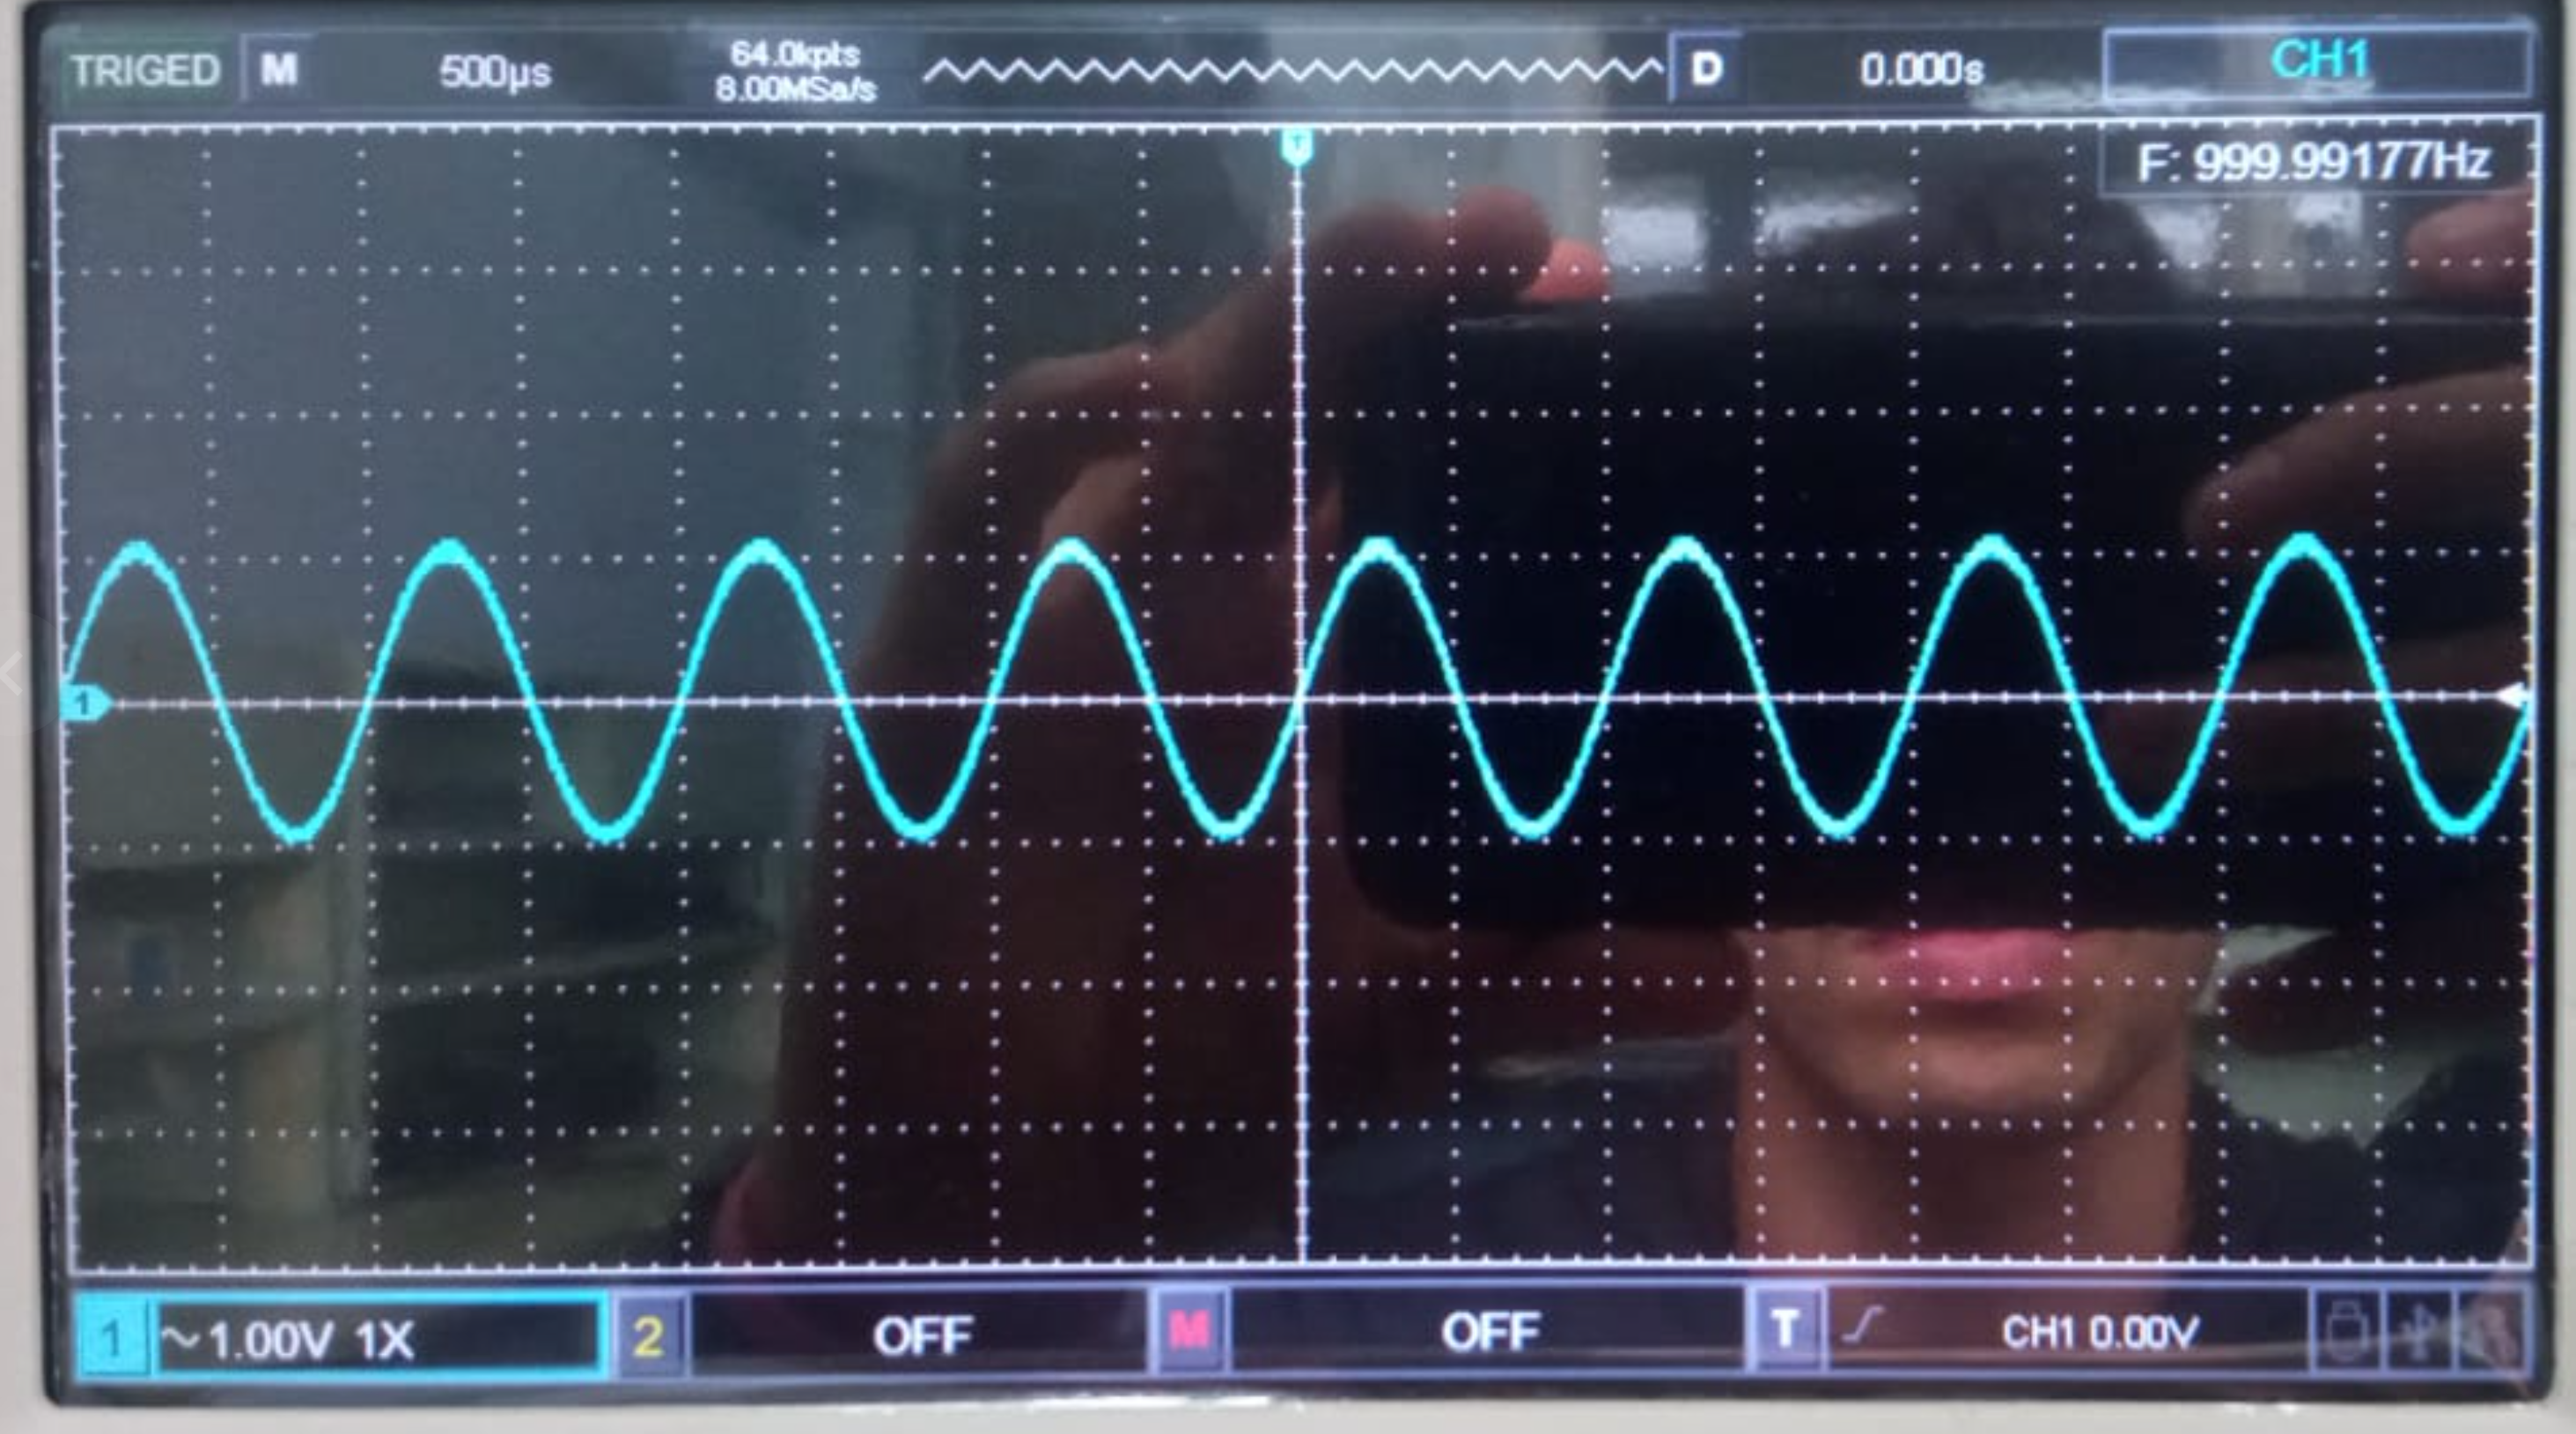
\includegraphics[width=\textwidth]{Imagenes/vinmulti.png}
                  \caption{Voltaje de entrada del amplificador multietapas}
                  \label{fig:vinmulti}
                \end{figure}

                \begin{table}[H]
                  \centering
                  \begin{tabular}{|c|c|c|c|}
                    \hline
                    \textbf{time/div} $[\mu s]$ & \textbf{Channel} & \textbf{voltios/div $[\volt]$} & \textbf{Acoplamiento} \\ \hline
                    $500 \, \pm 100 \, $        & 1 (Azul)         & $1 \pm 0.2  $                  & AC                    \\ \hline
                  \end{tabular}
                  \caption{Escalas Usada en el Osciloscopio Digital UNI-T UTD2102CEX+}
                  \label{tab:escala_vinmulti}
                \end{table}

          \item \textbf{Voltaje de salida en modo diferencial}

                \begin{figure}[H]
                  \centering
                  \renewcommand{\figurename}{Imagen}
                  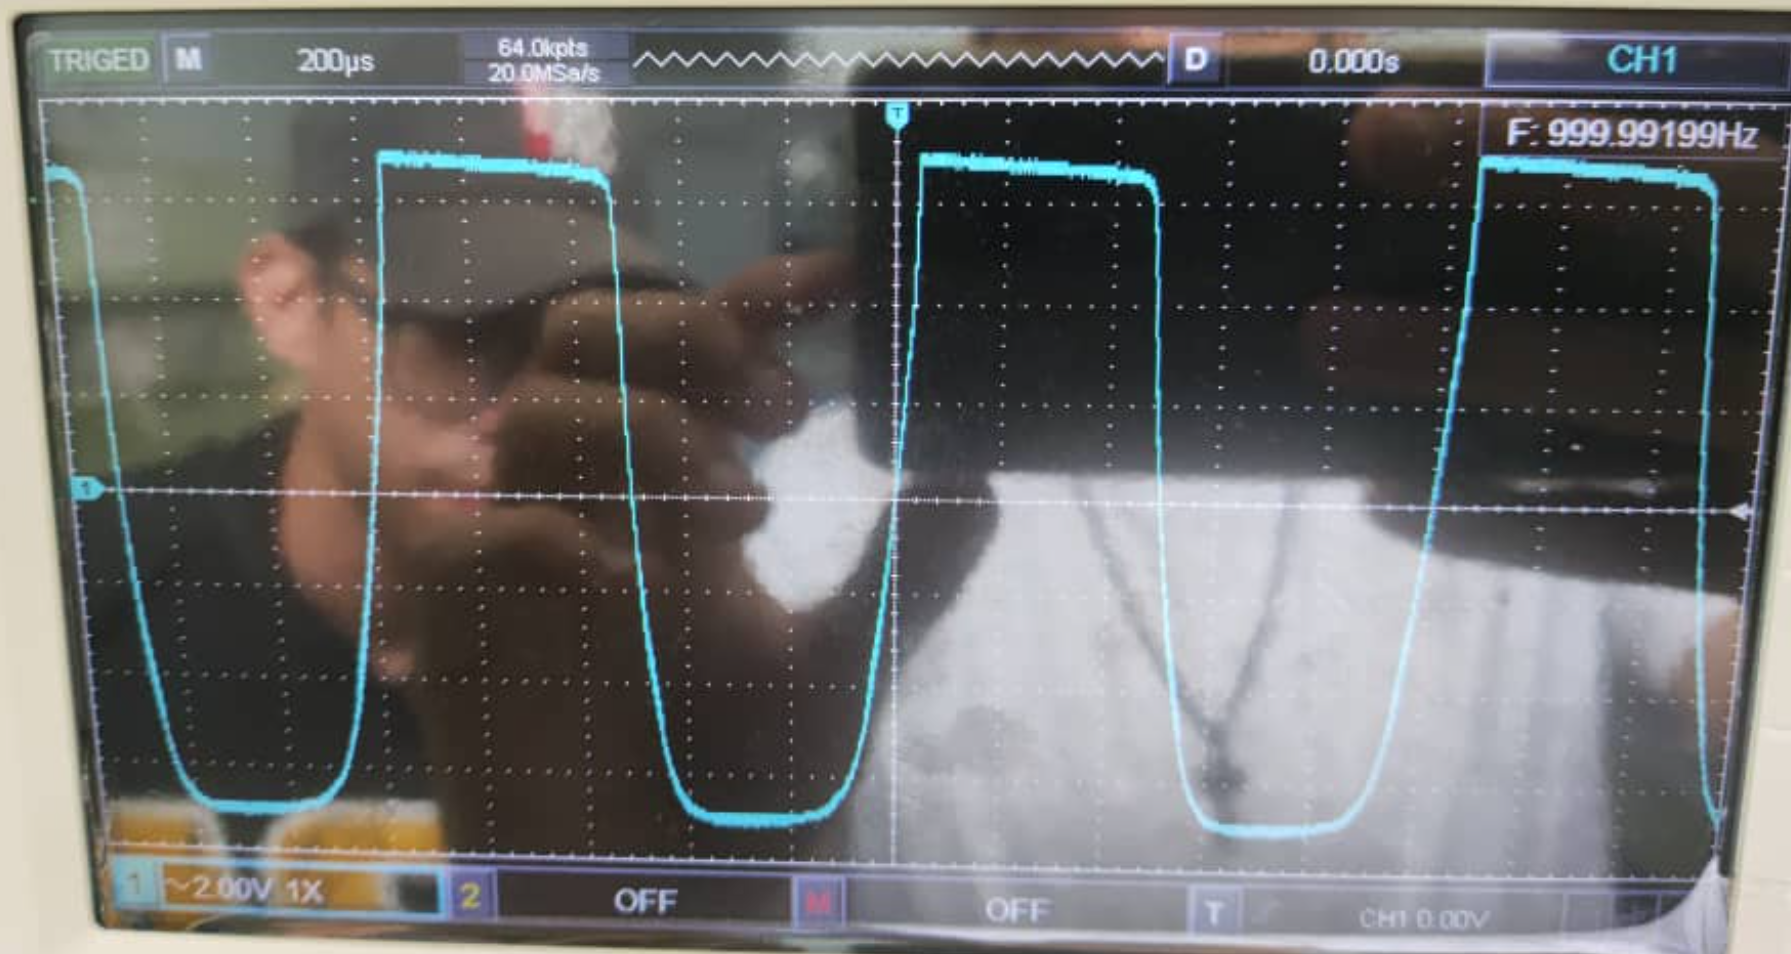
\includegraphics[width=\textwidth]{Imagenes/vodmultietapas.png}
                  \caption{Voltaje de salida del amplificador multietapas modo diferencial}
                  \label{fig:vodmultietapas}
                \end{figure}

                \begin{table}[H]
                  \centering
                  \begin{tabular}{|c|c|c|c|}
                    \hline
                    \textbf{time/div} $[\mu s]$ & \textbf{Channel} & \textbf{voltios/div $[\volt]$} & \textbf{Acoplamiento} \\ \hline
                    $200 \, \pm 40 \, $         & 1 (Azul)         & $2 \pm 0.4  $                  & AC                    \\ \hline
                  \end{tabular}
                  \caption{Escalas Usada en el Osciloscopio Digital UNI-T UTD2102CEX+}
                  \label{tab:escala_vodmultietapas}
                \end{table}

          \item \textbf{Voltaje de salida en modo común}
                \begin{figure}[H]
                  \centering
                  \renewcommand{\figurename}{Imagen}
                  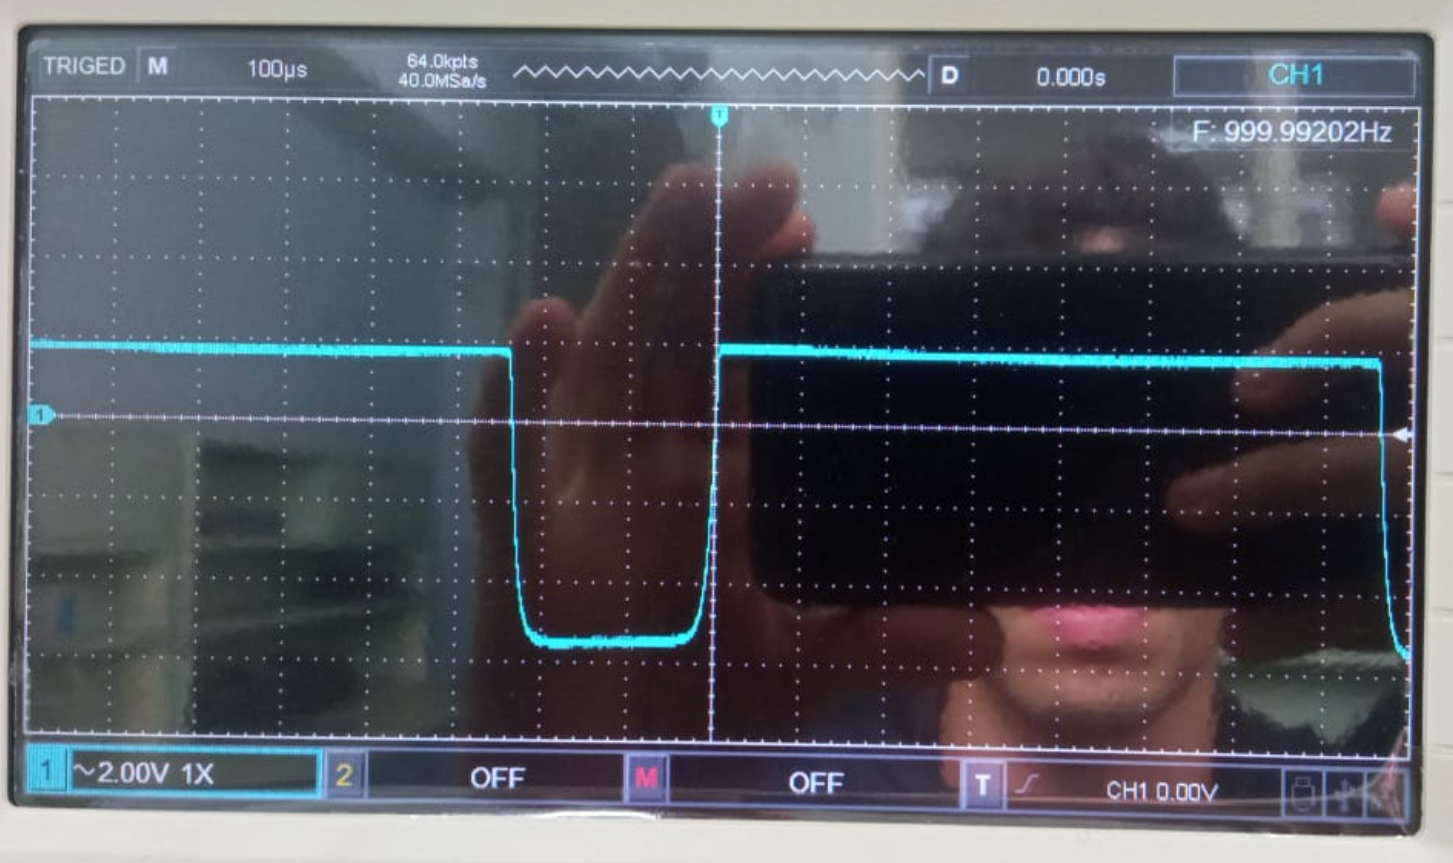
\includegraphics[width=\textwidth]{Imagenes/vocmulti.png}
                  \caption{Voltaje de salida del amplificador multietapas modo Común}
                  \label{fig:vocmulti}
                \end{figure}

                \begin{table}[H]
                  \centering
                  \begin{tabular}{|c|c|c|c|}
                    \hline
                    \textbf{time/div} $[\mu s]$ & \textbf{Channel} & \textbf{voltios/div $[\volt]$} & \textbf{Acoplamiento} \\ \hline
                    $200 \, \pm 40 \, $         & 1 (Azul)         & $2 \pm 0.4  $                  & AC                    \\ \hline
                  \end{tabular}
                  \caption{Escalas Usada en el Osciloscopio Digital UNI-T UTD2102CEX+}
                  \label{tab:escala_vocmulti}
                \end{table}

                Se observan las salidas de esa manera, debido a que tenemos una ganancia muy grande para el nivel de voltaje que se le dio en la entrada que era una de 1V, sin embargo se realizo con un voltaje de 5mV (ver tabla \ref{tab:ganancia_multietapas}), permitiendo ver la ganancia en zona lineal del amplificador multietapas.

        \end{itemize}
\end{enumerate}

\subsection{Parte 4. Respuesta en frecuencia}\label{subsec:parte4}

\begin{enumerate}
  \item \textbf{Determine experimentalmente los puntos de operación de los elementos activos, con el fin de verificar el correcto funcionamiento.}

        \begin{table}[H]
          \centering
          \begin{tabular}{|c|c|c|c|c|c|c|}
            \hline
            \textbf{Transistor} & \textbf{Vc[V]} & $\mathbf{\Delta Vc[V]}$ & \textbf{Vb[V]} & $\mathbf{\Delta Vb[V]}$ & \textbf{Ve[V]} & $\mathbf{\Delta Ve[V]}$ \\ \hline
            Q1                  & 7.2            & $\pm 0.4$               & 240m           & $\pm 20m$               & -360m          & $\pm 100m$              \\ \hline
            Q2                  & 7.2            & $\pm 0.4$               & 260m           & $\pm 20m$               & -360m          & $\pm 20m$               \\ \hline
            Q3                  & 5.2            & $\pm 0.4$               & 8              & $\pm 0.4$               & 9              & $\pm 1$                 \\ \hline
            Q4                  & 900m           & $\pm 100m$              & 360m           & $\pm 20m$               & -200m          & $\pm 20m$               \\ \hline
            Q5                  & 10             & $\pm 1$                 & 900m           & $\pm 100m$              & 380m           & $\pm 20m$               \\ \hline
            Q6                  & -10            & $\pm 1$                 & -220m          & $\pm 20m$               & 360m           & $\pm 20m$               \\ \hline
          \end{tabular}
          \caption{Mediciones para hallar punto de operación, acoplando sus etapas}
          \label{tab:punto_operacion4_aco}
        \end{table}



        Haciendo uso de las ecuaciones \ref{eqn:incertidumbre_vce} y \ref{eqn:incertidumbre_ic}, hallamos sus puntos de operación e incertidumbres (Acoplado).

        \begin{itemize}
          \item $\mathbf{V_{CEQ}}$

                \begin{align*}
                  V_{CEQ_3} & =5.2-(9)=-3.8 \pm 1.08\volt    \\[0.2cm]
                  V_{CEQ_1} & =7.2-(0.36)=7.56 \pm 0.41\volt \\[0.2cm]
                  V_{CEQ_2} & =7.2-(0.36)=7.56 \pm 0.41\volt \\[0.2cm]
                  V_{CEQ_4} & =0.9-(-0.2)=1.1 \pm 0.10\volt  \\[0.2cm]
                  V_{CEQ_5} & =10-(0.38)=9.62 \pm 1\volt     \\[0.2cm]
                  V_{CEQ_6} & =-10-(0.36)=-10.36 \pm 1\volt  \\[1cm]
                \end{align*}


          \item $\mathbf{I_{CQ}}$

                \begin{align*}
                  I_{CQ_3} & =\dfrac{9-(-10)}{6.8k}=2.79 \pm 0.25 mA                   \\[0.2cm]
                  I_{CQ_4} & =\dfrac{10-(-0.36)}{5k}=357.04 \pm 47.12\mu A             \\[0.2cm]
                  I_{CQ_5} & =\dfrac{10-(0.9)}{22k}=413.64 \pm 50.14\mu A              \\[0.2cm]
                  I_{CQ_6} & =\dfrac{-0.22-(-10)}{22k}=444.55 \pm 50.61\mu A           \\[0.2cm]
                  I_{CQ_1} & = I_{CQ_2}=\dfrac{10-(7.2)}{4.7k}=595.74 \pm 231.08 \mu A \\[1cm]
                \end{align*}



                \begin{table}[H]
                  \centering
                  \begin{tabular}{|c|c|c|c|c|c|c|}
                    \hline
                    \textbf{Transistores} & $v_{CE} [V]$ & $\Delta V_{CE} [V]$ & $E_{r_{V_{CE}}} [\%]$ & $I_{C} [\mu A]$ & $\Delta I_{C} [\mu A]$ & $E_{r_{I_{C}}} [\%]$ \\
                    \hline
                    $Q_1$                 & $7.56$       & $\pm 0.41 $         & $5.5$                 & $595.74$        & $\pm 231.08$           & $1.67$               \\
                    \hline
                    $Q_2$                 & $7.56$       & $\pm 0.40 $         & $5.5$                 & $595.74$        & $\pm 231.08$           & $1.67$               \\
                    \hline
                    $Q_3$                 & $-3.8$       & $\pm 1.08$          & $17.48$               & $2790$          & $\pm 250$              & $24.55$              \\
                    \hline
                    $Q_4$                 & $1.1$        & $\pm 0.10$          & $15.38$               & $357.04$        & $\pm 47.12$            & $21.03$              \\
                    \hline
                    $Q_5$                 & $9.62$       & $\pm 1.00$          & $3.8$                 & $413.64$        & $\pm 50.14$            & $3.96$               \\
                    \hline
                    $Q_6$                 & $-10.36$     & $\pm 1.00$          & $3.6$                 & $444.55$        & $\pm 50.61$            & $11.73$              \\
                    \hline
                  \end{tabular}
                  \caption{Mediciones indirectas con sus errores relativos de sus puntos de operación Acoplados}
                  \label{tab:puntos_operacion_experimental_maserror_parte34}
                \end{table}

        \end{itemize}

  \item \textbf{Utilizado la metodología expuesta por Ud. en el trabajo
          previo, determinar experimentalmente: las frecuencias
          de corte inferior y superior del amplificador y la ganancia a frecuencias medias.}
  \item \textbf{Basándose en la metodología para obtener la respuesta
          en frecuencia, expuesta por Ud. en el trabajo previo, determine la ganancia del amplificador, para
          aproximadamente cada una de las frecuencias seleccionadas.
          Para reportarlas construya el gráfico experimental
          correspondiente, superponiéndolo a la respuesta
          en frecuencia esperada y al diagrama de Bode asintótico.}

        En este apartado en particular, cada una de las mediciones fueron realizadas a traves de los valores dados por el osciloscopio marca: Unit, modelo: UTD2102CEX+, donde se uso la función \textbf{All Parameter}, que permite ser mas precisos en su lectura, usándola de forma adecuada, por esa razón, se usara las incertidumbres dadas por el fabricante del osciloscopio en el manual de usuario, que se halla en la sección \ref{sec:apendice}, las ecuaciones \ref{eqn:delta_t} y \ref{eqn:delta_v}.


        \begin{table}[H]
          \centering
          \begin{tabular}{|c|c|c|c|c|c|c|c|c|c|}
            \hline
            \textbf{f[Hz]} & $\mathbf{\Delta f [Hz]}$ & \textbf{T [s]} & $\mathbf{\Delta T [s]}$ & \textbf{Vi[V]} & $\mathbf{\Delta Vi[V]}$ & \textbf{Vo[V]} & $\mathbf{\Delta Vo[V]}$ & \textbf{Ad[V/V]} & $\mathbf{\Delta Ad[V/V]}$ \\
            \hline
            40             & $\pm1.616$               & 25 m           & $\pm 1.01m$             & 20m            & $\pm 1.1m$              & 200m           & $\pm 11m$               & 10               & $\pm 0.55$                \\
            \hline
            50             & $\pm 2.525$              & 20m            & $\pm 1.01m$             & 20m            & $\pm 1.1m$              & 300m           & $\pm 14m$               & 15               & $\pm 0.7$                 \\
            \hline
            61             & $\pm 3.758$              & 16.393 m       & $\pm 1.01m$             & 20m            & $\pm 1.1m$              & 270 m          & $\pm 13.1m$             & 13.5             & $\pm 0.66$                \\
            \hline
            100            & $\pm 4$                  & 9.99 m         & $\pm 0.4 m$             & 20m            & $\pm 1.1m$              & 600m           & $\pm 23m$               & 30               & $\pm 1.15$                \\
            \hline
          \end{tabular}
          \caption{Mediciones de ganancia en modo diferencial en el multietapas con frecuencias bajas Acoplado}
          \label{tab:ganancia_frecuencias_bajas}
        \end{table}


        \begin{table}[H]
          \centering
          \begin{tabular}{|c|c|c|c|c|c|c|c|c|c|}
            \hline
            \textbf{f[Hz]} & $\mathbf{\Delta f [Hz]}$ & \textbf{T [s]} & $\mathbf{\Delta T [s]}$ & \textbf{Vi[V]} & $\mathbf{\Delta Vi[V]}$ & \textbf{Vo[V]} & $\mathbf{\Delta Vo[V]}$ & \textbf{Ad[V/V]} & $\mathbf{\Delta Ad[V/V]}$ \\
            \hline
            300            & $\pm 36$                 & 3.34 m         & $\pm 0.4m$              & 20m            & $\pm 1.1m$              & 1              & $\pm 40m$               & 50               & $\pm 2.00$                \\
            \hline
            370            & $\pm 54.76$              & 2.70m          & $\pm 0.4m$              & 20m            & $\pm 1.1m$              & 1              & $\pm 40m$               & 50               & $\pm 2.00$                \\
            \hline
            500            & $\pm 100$                & 2m             & $\pm 0.4m$              & 20m            & $\pm 1.1m$              & 1              & $\pm 40m$               & 50               & $\pm 2.00$                \\
            \hline
            1k             & $\pm 40.5$               & 1m             & $\pm 40.5 \mu$          & 20m            & $\pm 1.1m$              & 1              & $\pm 40m$               & 50               & $\pm 2.00$                \\
            \hline
            5k             & $\pm 252.5$              & $200 \mu$      & $\pm 10.10 \mu$         & 20m            & $\pm 1.1m$              & 1              & $\pm 40m$               & 50               & $\pm 2.00$                \\
            \hline
            10k            & $\pm 405$                & $100 \mu$      & $\pm 4.05 \mu$          & 20m            & $\pm 1.1m$              & 1              & $\pm 40m$               & 50               & $\pm 2.00$                \\
            \hline
          \end{tabular}
          \caption{Mediciones de ganancia en modo diferencial en el multietapas con frecuencias medias Acoplado}
          \label{tab:ganancia_frecuencias_medias}
        \end{table}


        \begin{table}[H]
          \centering
          \begin{tabular}{|c|c|c|c|c|c|c|c|c|c|}
            \hline
            \textbf{f[Hz]} & $\mathbf{\Delta f [Hz]}$ & \textbf{T [s]} & $\mathbf{\Delta T [s]}$ & \textbf{Vi[V]} & $\mathbf{\Delta Vi[V]}$ & \textbf{Vo[V]} & $\mathbf{\Delta Vo[V]}$ & \textbf{Ad[V/V]} & $\mathbf{\Delta Ad[V/V]}$ \\
            \hline
            14k            & $\pm 399.84$             & $71.43 \mu$    & $\pm 2.04 \mu$          & 20m            & $\pm 1.1m$              & 1              & $\pm 40m$               & 50               & $\pm 2.00$                \\
            \hline
            20k            & $\pm 812$                & $50 \mu$       & $\pm 2.03 \mu$          & 20m            & $\pm 1.1m$              & 1              & $\pm 40m$               & 50               & $\pm 2.00$                \\
            \hline
            33k            & $\pm 2.2 k$              & $3.3 \mu$      & $\pm 2.02 \mu$          & 20m            & $\pm 1.1m$              & 950 m          & $\pm 38.5m$             & 47.5             & $\pm 1.93$                \\
            \hline
            40k            & $\pm 1.616k$             & $25 \mu$       & $\pm 1.01 \mu$          & 20m            & $\pm 1.1m$              & 900m           & $\pm 37m$               & 45               & $\pm 1.85$                \\
            \hline
            45k            & $\pm 2.045k$             & $22.2 \mu$     & $\pm 1.01 \mu$          & 20m            & $\pm 1.1m$              & 850 m          & $\pm 35.5m$             & 42.5             & $\pm 1.78$                \\
            \hline
            55k            & $\pm 3.055k$             & $18.18 \mu$    & $\pm 1.01 \mu$          & 20m            & $\pm 1.1m$              & 750m           & $\pm 27.5m$             & 37.5             & $\pm 1.38$                \\
            \hline
            75k            & $\pm 2.306k$             & $13.3\mu$      & $\pm 0.41 \mu$          & 20m            & $\pm 1.1m$              & 600m           & $\pm 23m$               & 30               & $\pm 1.15$                \\
            \hline
            145k           & $\pm 4.205k$             & $6.89 \mu$     & $\pm0.2\mu$             & 20m            & $\pm 1.1m$              & 300            & $\pm 14m$               & 15               & $\pm 0.7$                 \\
            \hline
            180k           & $\pm 6.48k$              & $5.5 \mu$      & $\pm 0.2\mu$            & 20m            & $\pm 1.1m$              & 250            & $\pm 12.5m$             & 12.5             & $\pm 0.63$                \\
            \hline
          \end{tabular}
          \caption{Mediciones de ganancia en modo diferencial en el multietapas con frecuencias altas Acoplado}
          \label{tab:ganancia_frecuencias_altas}
        \end{table}




        \begin{table}[H]
          \centering
          \begin{tabular}{|c|c|c|}
            \hline
            $\mathbf{f_L[Hz]}$ & $\mathbf{f_H[Hz]}$ \\ \hline
            60                 & 20k                \\ \hline
          \end{tabular}
          \caption{Frecuencias de corte del circuito amplificador multietapas}
          \label{tab:frecuencias_corte}
        \end{table}

        \begin{figure}[H]
          \centering
          \setcounter{figure}{54}
          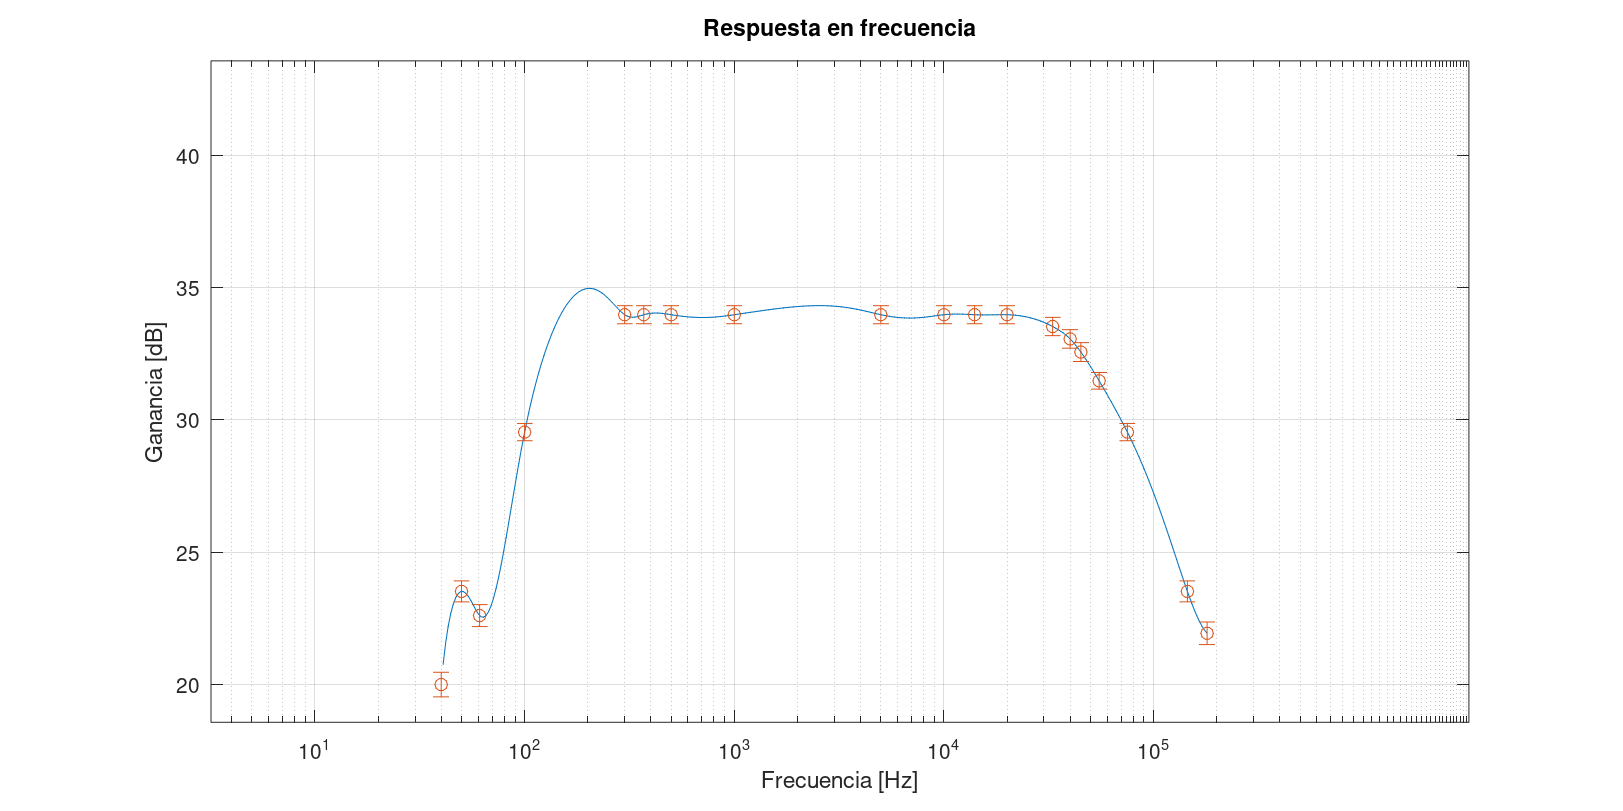
\includegraphics[width=\textwidth]{Imagenes/bode.png}
          \caption{Diagrama experimental de bode de magnitud}
          \label{fig:bode}
        \end{figure}
\end{enumerate}

\subsection{Parte 5. Realimentación} \label{subsec:parte5}


\begin{enumerate}

  \item \textbf{Practique en el amplificador base la realimentación
          negativa que se indica en la sección de preparación.
          Observe el efecto de cruce y repórtelo mediante gráfico o fotografía.}

        \begin{figure}[H]
          \centering
          \renewcommand{\figurename}{Imagen}
          \setcounter{figure}{8}
          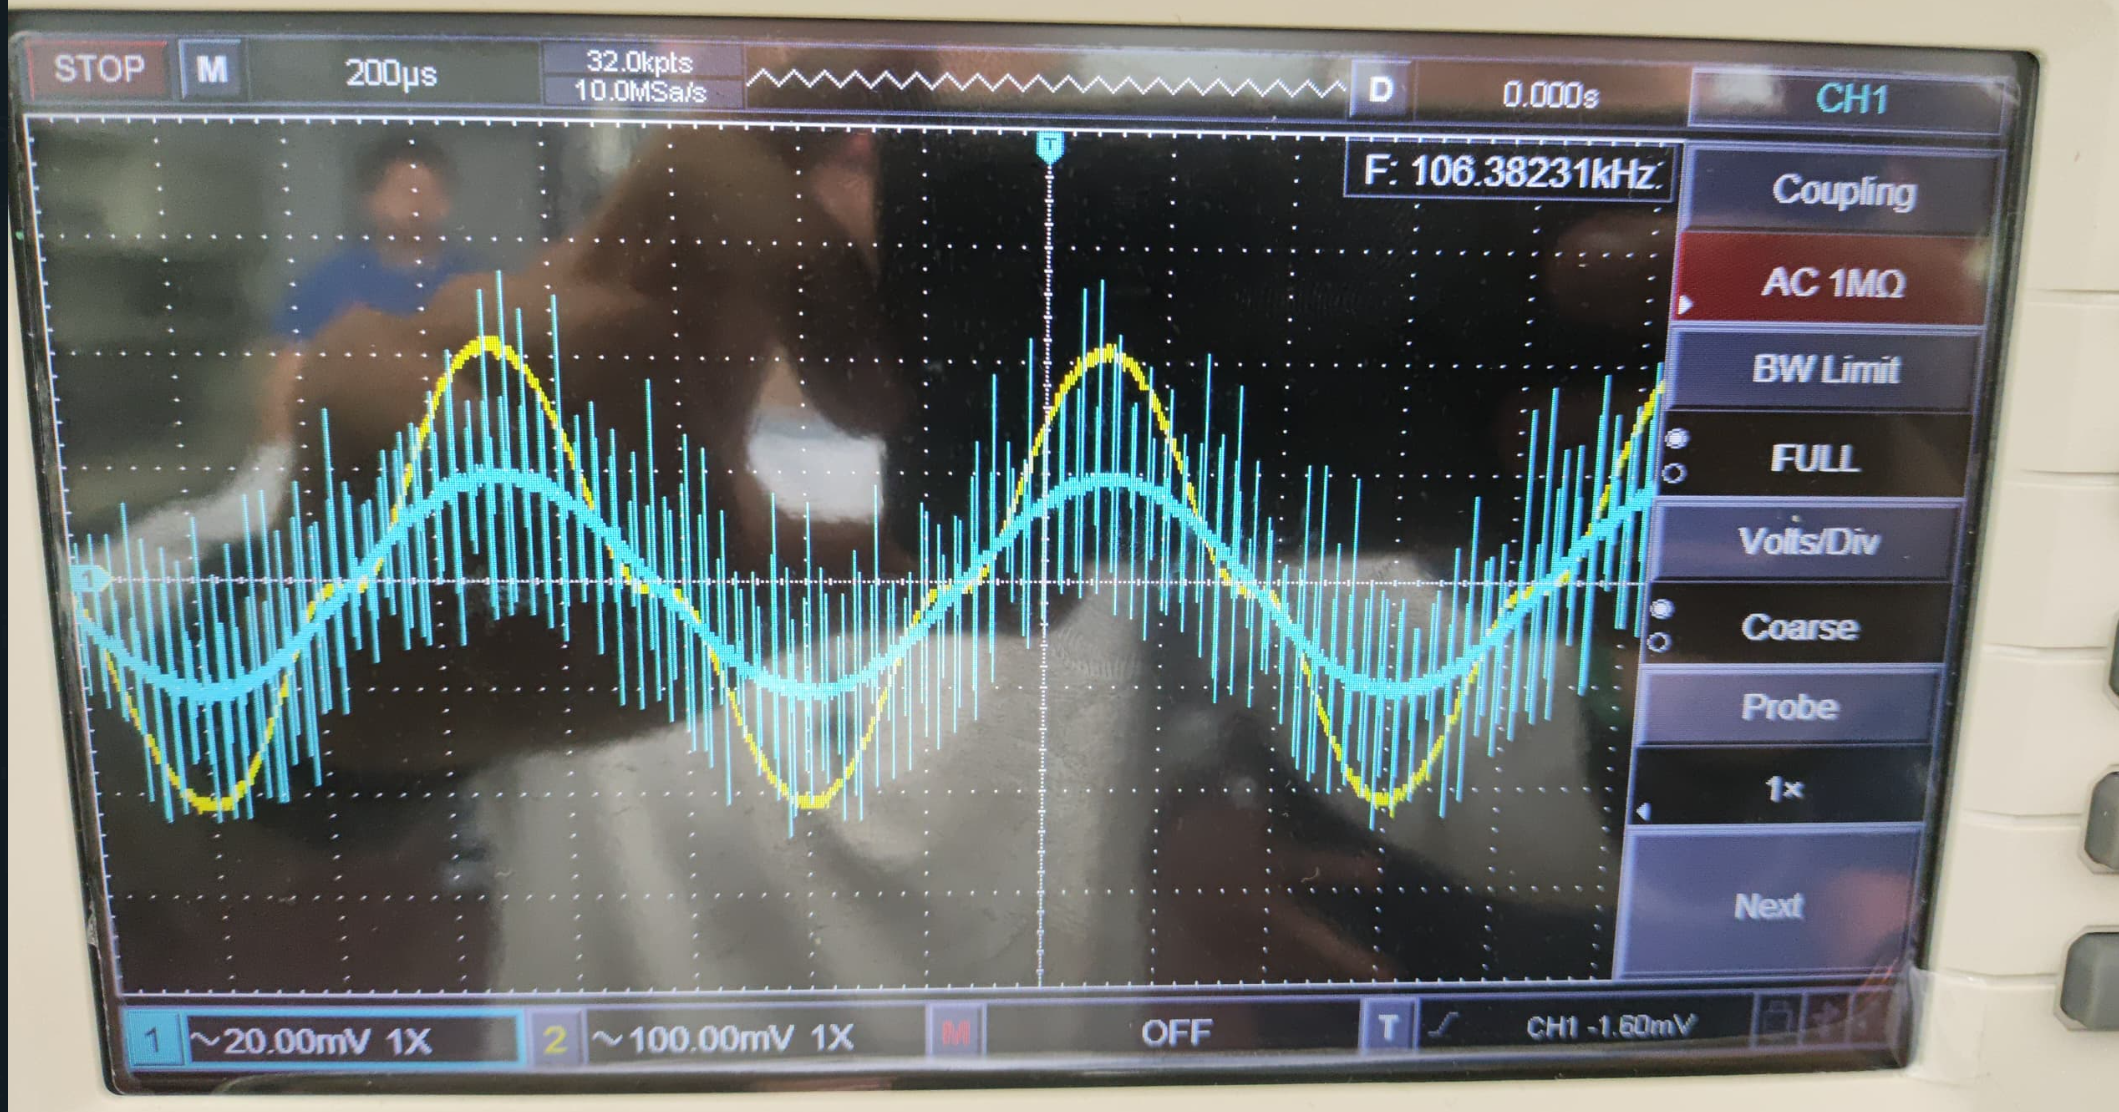
\includegraphics[width=\textwidth]{Imagenes/ultcrossover.png}
          \caption{efecto de crossover con retroalimentación}
          \label{fig:ultcross}
        \end{figure}

  \item \textbf{Para el circuito realimentado negativamente, determine experimentalmente: las Impedancias de entrada
          y salida, la Ganancia a frecuencias medias y las frecuencias
          de corte. Por último mida la Respuesta en frecuencia.}

        \begin{table}[H]
          \centering
          \begin{tabular}{|c|c|}
            \hline
            $\mathbf{f_L[Hz]}$ & $\mathbf{f_H[Hz]}$ \\ \hline
            60                 & 20k                \\ \hline
          \end{tabular}
          \caption{Frecuencias de corte del circuito amplificador multietapas}
          \label{tab:frecuencias_corte1}
        \end{table}

        \begin{table}[H]
          \centering
          \begin{tabular}{|c|c|c|c|c|c|c|c|}
            \hline
            $V_g[V]$ & $\Delta V_g[V]$ & $V_i[V]$ & $\Delta V_i[V]$ & $R_p[\Omega]$ & $\Delta R_p[\Omega]$ & $Z_d[\Omega]$ & $\Delta Z_d[\Omega]$ \\ \hline
            20m      & $\pm 4m$        & 1m       & $\pm 0.25m$     & 47k           & $\pm 5\%$            & 49.5k         & $\pm 253.878$        \\ \hline
          \end{tabular}
          \caption{Medición de impedancia de entrada en modo diferencial en el multietapas}
          \label{tab:impedancia_entrada_diferencial1}
        \end{table}

        \begin{table}[H]
          \centering
          \begin{tabular}{|c|c|c|c|c|c|c|c|}
            \hline
            $Vo_{sc}[V]$ & $\Delta Vo_{sc}[V]$ & $Vo_{cc}[V]$ & $\Delta Vo_{cc}[V]$ & $R_p[\Omega]$ & $\Delta R_p[\Omega]$ & $Z_o[\Omega]$ & $\Delta Z_o[\Omega]$ \\ \hline
            400m         & $\pm 20m$           & 50m          & $\pm 10m$           & 15            & $\pm 5\%$            & 105           & $\pm 12.75$          \\ \hline
          \end{tabular}
          \caption{Medición de impedancias de Salida}
          \label{tab:impedancias_salida11}
        \end{table}

        \begin{table}[H]
          \centering
          \begin{tabular}{|c|c|c|c|c|c|c|}
            \hline
            $f[Hz]$ & $Vi[V]$ & $\Delta Vi[V]$ & $Vo[V]$ & $\Delta Vo[V]$ & $Ad[V/V]$ & $\Delta Ad[V/V]$ \\ \hline
            1k      & 20m     & $\pm 4m$       & 400m    & $\pm 20m$      & 20        & $\pm 4.123$      \\ \hline
          \end{tabular}
          \caption{Mediciones de ganancia en modo diferencial en el multietapas con frecuencias medias}
          \label{tab:ganancia_diferencial_medias11}
        \end{table}
  \item \textbf{Practique al amplificador base la realimentación positiva que se indica en la sección de preparación y
          gráfica o fotografié la señal de salida y compare con
          el resultado de la simulación realizada en trabajo previo.}

        \begin{figure}[H]
          \centering
          \renewcommand{\figurename}{Imagen}
          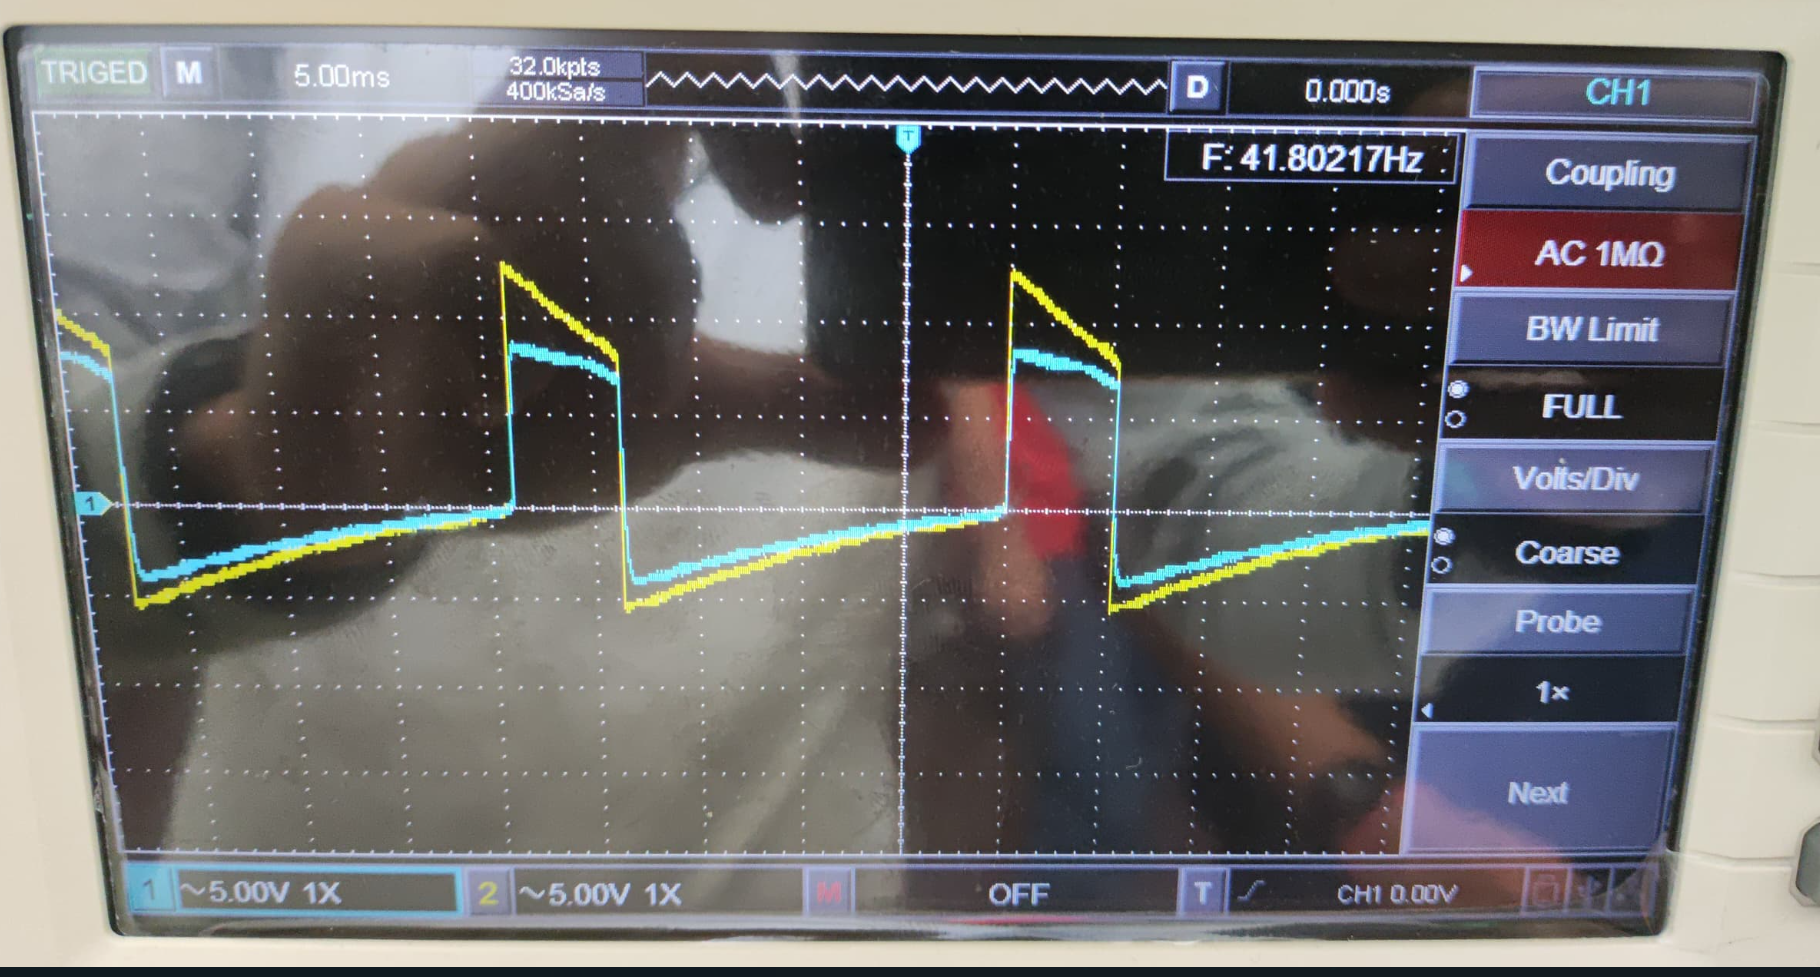
\includegraphics[width=\textwidth]{Imagenes/realimentacionpositiva.png}
          \caption{realimentación positiva y negativa, generando una oscilación}
          \label{fig:realimentacionpositiva}
        \end{figure}

\end{enumerate}


\newpage